\chapter{Modeling Photovoltaics}\label{chapter:modeling_pvs}

In this chapter, \textbf{Modeling Photovoltaics}, we systematically review the
various types of abstractions in photovoltaics, starting from solar cells and
ending with solar arrays.

We start by observing how solar cell models can have differing granularities in
their composition and in how they address an array of internal qualities and
external environs that influence real world performance. Alongside defining
these models, we also propose modifications that may improve their accuracy and
precision, and consider tradeoffs that may occur in nonnominal conditions. After
defining these models, we then present an in-depth methodology for evaluating
them; we construct a dataset of solar cell \ac{I-V} curves characterized for use
on the \ac{LHRs} solar vehicle, then define techniques for extracting model
parameters for each cell. We proceed to use those model parameters to predict
their behavior in different conditions, and evaluate how they perform in terms
of model accuracy and precision.

We select the `best' set of solar cell models and use them as
building blocks to build larger models, namely those for solar modules. These
solar modules can take multiple shapes and sizes, and may exhibit reverse bias
behavior in the event of photovoltaic mismatch, a phenomenon caused by
nonuniform cells in series or in parallel. We also extend the module model by
adding a bypass diode in antiparallel, and discussing how solar cell reverse
bias behavior may drive their turn on conditions and mismatch mitigation
effects. From these solar module models, we formulate a metric to measure
mismatch, and propose suggestions and observations on how module size and cell
characteristics may influence the total efficiency of the module. Insights
developed in this section will later on become heuristics and algorithms for
optimizing module design in \autoref{chapter:optimizing_pvs}. We extend the test
methodology used for evaluating solar cells to solar modules, and validate
whether the module models pass muster.

% , either through manufacturing defects
% or lighting and thermal gradients across the module.

Finally, we take these solar module models and combine them together to form a
cohesive solar array model. From this model, we observe how the individual
module effects can generate a global \ac{I-V} curve with local and global
maxima, and discuss how this curve impacts the way the larger photovoltaic
system interacts with solar arrays. We also perform array testing using the
\ac{LHRs} solar array, and compare a simulated version of the array test with
real world data to determine a final, holistic evaluation of the models used.

\section{Modeling Solar Cells}\label{sec:modeling_solar_cells}

In this thesis, we will discuss three solar cell model abstractions:

\begin{itemize}
    \item Three Parameter Solar Cell Model (Single Diode Model)
    \item Five Parameter Solar Cell Model (Complete Single Diode Model)
    \item Seven Parameter Solar Cell Model (Double Diode Model)
\end{itemize}

To restrain the breadth of this document, we'll focus on the aforementioned
three models, since they are the most commonly cited and used abstractions. That
is not to diminish the dozens, if not hundreds more types of solar cell models,
like the three diode model proposed by Khanna et al~\cite{khanna_et_al}, or the
Bishop model with an avalanche breakdown
component~\cite{restrepo_cuestas_et_al}, or the \acf{DRM} that utilizes
antiparallel diode-resistor paths~\cite{restrepo_cuestas_et_al}.

\subsection{Three Parameter Solar Cell Model}\label{subsec:three_parameter_solar_cell_model}

\begin{figure}[h]
    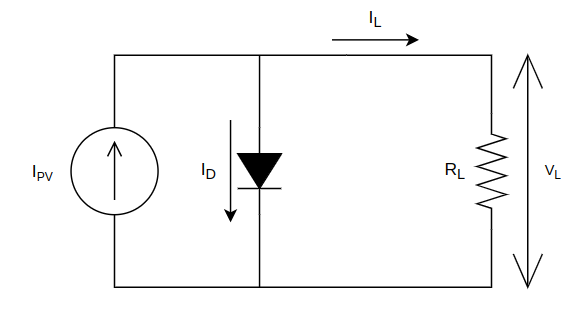
\includegraphics[width=\textwidth]{solar_cell_three_parameter_model.png}
    \caption{Three Parameter, or Single Diode Model of a Solar Cell}
    \label{fig:single_diode_model}
\end{figure}

The most basic model of a solar cell is the three parameter model, or single
diode model, shown in \autoref{fig:single_diode_model}. It consists of a
constant current source and a diode. The constant current source produces a
\ac{IPV} caused by photons of sufficient energy being absorbed into the surface
of the solar cell and exciting charge carriers (generally in the form of
electrons) to enter the circuit. The diode represents the various recombination
processes that consume the generated current in the form of \ac{ID}.

In this model, the three parameters consist of the following:

\begin{itemize}
    \item \acf{IPV},
    \item \acf{I0},
    \item and an \acf{N}.
\end{itemize}

The latter two are contained within the dark current term, and generally
influence the shape of the predicted \ac{I-V} curve, particularly around the
knee-bend.

This model is juxtaposed from the five parameter model in that it does not
incorporate cell losses in the form of \ac{RS} and \ac{RSH}. It is assumed that
in this model, the series resistance is zero (short circuit) and the shunt
resistance is infinite (open circuit). Therefore, the five parameter model may
also be called the complete single diode model.

We observe from \autoref{fig:single_diode_model} that the \ac{IL} can be
represented as a function of the photocurrent and the dark current
(\autoref{eq:cell_output_current_1}).

\begin{equation}
    I_L = I_{PV} - I_D
    \equnit{\si{\ampere}}
    \label{eq:cell_output_current_1}
\end{equation}

In the following text, we break down each component into its constituent parts.


\subsubsection{Photocurrent}\label{subsubsec:three_param_photocurrent}

\begin{equation}
    I_{PV} = qA\int_{}{}b_s(E)QE(E)dE
    \equnit{\si{\ampere}}
    \label{eq:cell_photocurrent_1}
\end{equation}

On a fundamental level, we can define the \acf{IPV} as a function of the photons
incident upon the surface of the solar cell and the solar cell's spectral
response. This is demonstrated in \autoref{eq:cell_photocurrent_1}. A bulleted,
simplistic explanation of this equation is presented as follows:

\begin{itemize}
    \item Incident light hits the solar cell over a given spectrum of energy
    levels (denoted either in $eV$ or in $nm$) (see
    \autoref{fig:maxeon_gen_iii_cell_spectral_response}).
    \item Incident light at each discrete energy level has an \ac{BS}, otherwise
    known as intensity.
    \item The solar cell has a given \ac{QE} at each energy level that is the
    probability that an incident photon of \ac{E} delivers one electron to the
    external circuit.
    \item Integrating the product of the photon flux density \ac{BS} and quantum
    efficiency \ac{QE} (then multiplied by the \ac{Q} and the cell \ac{A})
    provides the photocurrent (\ac{IPV}).
\end{itemize}

\begin{figure}[h]
    \center
    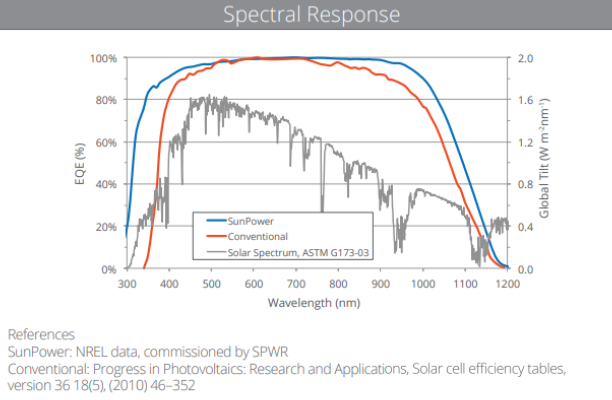
\includegraphics[width=0.95\textwidth]{maxeon_gen_iii_cell_spectral_response.png}
    \caption{Maxeon Gen III Cell Spectral Response}
    \label{fig:maxeon_gen_iii_cell_spectral_response}
\end{figure}

Solar cell manufacturers may provide a spectral response chart showing the
quantum efficiency over the useful solar spectrum, as seen in
\autoref{fig:maxeon_gen_iii_cell_spectral_response}, but will generally just
provide the \ac{ISC} at \ac{STC} ($1000$ $Wm^{-2}$, $AM$ $1.5G$, $25$ $C$).

As it turns out, the photocurrent can generally be approximated as the short
circuit current. We'll discuss in \autoref{subsubsec:five_param_series_resistance}
that Cubas et al.~\cites{cubas_et_al,cubas_et_al_2} defines the
photocurrent as a ratio of the series and shunt resistance in addition to the
short circuit current. However, in most cases, the empirical value of \acl{ISC}
will not differ from \autoref{eq:cell_photocurrent_2}.

\begin{equation}
    I_{PV} = I_{SC}
    \equnit{\si{\ampere}}
    \label{eq:cell_photocurrent_2}
\end{equation}


\subsubsection{Dark Current}\label{subsubsec:three_param_dark_current}

The \acf{ID} comprises of the interesting and critical parameters of the three
parameter model; shown in \autoref{eq:cell_dark_current_1}, it consists of the
term \ac{I0} and an exponential. The exponential is a function of three key
variables: the \acf{TC}, \acf{VL}, and \acf{N}.

\begin{equation}
    I_D = I_0 \left[\exp\left(\frac{V_L}{V_T}\right) - 1\right]
    \equnit{\si{\ampere}}
    \label{eq:cell_dark_current_1}
\end{equation}

\noindent
where

\begin{equation}
    V_T = \frac{n k_B T_C}{q}
    \equnit{\si{\volt}}
    \label{eq:cell_thermal_voltage}
\end{equation}

This ideality factor is typically between $1$ and $2$, and represents the
proportional influence of carriers in several recombination processes for a
given cell composition and structure. Some ideality factor values are presented
in \autoref{table:ideality_factors}, sourced from PVEducation's Ideality Factor
page~\cite{pveducation_ideality_factor}. We note that the ideality factor may be
outside the typical range of $[1, 2]$, as discussed by Jain et
Kapoor~\cite{jain_et_kapoor} and R.N. Hall~\cite{hall}, the latter of which
notes that auger recombination dominated dark currents may generate a \ac{N} of
$2/3$.

The term \ac{VT} (\autoref{eq:cell_thermal_voltage}) which encapsulates the cell
temperature dependency describes the voltage across the P-N junction of the
diode in the model: at \ac{STC} this is typically $26$ $mV$. We remind the
reader that the remaining terms in this equation are the \acf{KB} and \acf{Q}.

\begin{table}[h!]
    \begin{tabularx}{\textwidth}{
        | >{\raggedright\arraybackslash}X
        | >{\raggedright\arraybackslash}X
        | >{\raggedright\arraybackslash}X | }
        \hline
        Recombination Type & Ideality Factor & Description \\ \hline \hline
        SRH, band to band (low level injection) & 1 & Recombination limited by minority carrier. \\ \hline
        SRH, band to band (high level injection) & 2 & Recombination limited by both carrier types. \\ \hline
        Auger & 2/3 & Two majority and one minority carriers required for recombination. \\ \hline
        Depletion region (junction) & 2 & Two carriers limit recombination. \\ \hline
    \end{tabularx}
    \caption{Various Ideality Factors of \ac{N}}
    \label{table:ideality_factors}
\end{table}


\subsubsection{Dark Saturation Current}\label{subsubsec:three_param_dark_sat_current}

The \acf{I0} has two potential derivations. Generally, the three parameter
model, (see Baig et al.~\cite{baig_et_al}, MacAlpine et
Brandemuehl~\cite{macalpine_et_brandemuehl}, Rusirawan et
Farkas~\cite{rusirawan_et_farkas}, and others) define \ac{I0} as in
\autoref{eq:cell_dark_sat_current_1}; where the diode current is a function of
the cell temperature and the energy bandgap in relation to several reference
parameters at \ac{STC}.

\begin{equation}
    I_0 = I_{0,ref}{(\frac{T_C}{T_{C,ref}})}^3\exp(\frac{E_{G,ref}}{k_B T_{C,ref}} - \frac{E_G}{k_B T_C})
    \equnit{\si{\ampere}}
    \label{eq:cell_dark_sat_current_1}
\end{equation}

On the other hand, we can derive the \ac{I0} algebraically: given the short
\acf{ISC} and \ac{VOC}, we can set the cell at open circuit,
forming the derivation in \autoref{eq:cell_dark_sat_current_deriv} and the
result in \autoref{eq:cell_dark_sat_current_2}.

\begin{equation}
    \begin{split}
        I_L = 0 &= I_{SC} - I_D \\
        & = I_{SC} - I_0[\exp(\frac{V_{OC}}{V_T}) - 1]
    \end{split}
    \equnit{\si{\ampere}}
    \label{eq:cell_dark_sat_current_deriv}
\end{equation}

\noindent
which gives

\begin{equation}
    I_0 = I_{SC}[\exp(\frac{V_{OC}}{V_T}) - 1]^{-1}
    \equnit{\si{\ampere}}
    \label{eq:cell_dark_sat_current_2}
\end{equation}

The latter model is convenient since it does not require measuring \ac{I0REF},
\ac{EGREF}, nor \ac{EG}. As such, we will focus on the latter model in
\autoref{subsec:eval_solar_cell_models}.


\subsubsection{Short Circuit Current}\label{subsubsec:three_param_short_circuit_current}

Finally, for the three parameter model, we derive the dependence of \acf{ISC}
and \acf{VOC} on \acf{G} and \acf{TC} before establishing the final derivation
of \autoref{eq:cell_output_current_1}.

Starting with the \acf{ISC}, it is known that there is a large positive
correlation with irradiance and a small positive correlation with temperature,
shown in \autoref{fig:cell_temperature_dependence} and
\autoref{fig:cell_irradiance_dependence}.

\begin{figure}[!htbp]
    \centering
    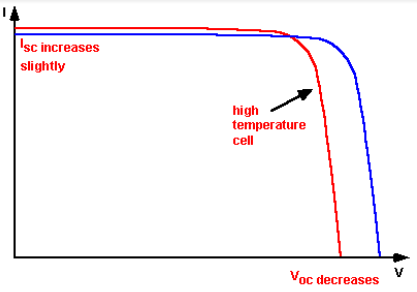
\includegraphics[width=0.7\linewidth]{cell_temperature_dependence.png}
    \caption{Solar Cell Temperature Dependence}
    \label{fig:cell_temperature_dependence}
\end{figure}

\begin{figure}[!htbp]
    \centering
    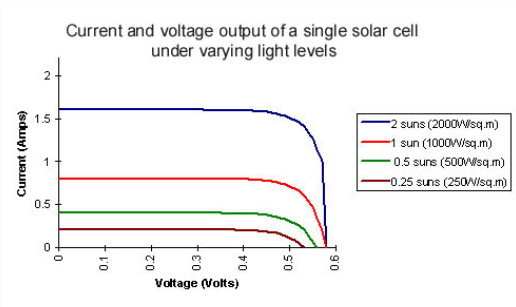
\includegraphics[width=0.9\linewidth]{cell_irradiance_dependence.png}
    \caption{Solar Cell Irradiance Dependence}
    \label{fig:cell_irradiance_dependence}
\end{figure}

The dependence of irradiance on $I_{SC}$ can be modeled as linearly proportional
to the light incident upon the solar cell over the reference irradiance. This
makes intuitive sense: given half the available light (assuming the distribution
of light across the spectrum is consistent), the solar cell will only be able to
capture half the maximum available power. Chegaar et al.~\cite{chegaar_et_al}
proposes this relationship as \autoref{eq:cell_short_circuit_current_1}, where
the short circuit current is a function of \ac{KE} and \acf{G} (the latter in
units of $Wm^{-2}$).

\begin{equation}
    I_{SC}(G) = K_E G
    \equnit{\si{\ampere}}
    \label{eq:cell_short_circuit_current_1}
\end{equation}

\autoref{eq:cell_short_circuit_current_1} can be easily reworked where the
constant \ac{KE} is now based on a \acf{ISCREF} and a \ac{GREF}. This forms
\autoref{eq:cell_short_circuit_current_2}, which is the same form used by Baig
et al.~\cite{baig_et_al}.

\begin{equation}
    I_{SC}(G) = I_{SC,ref}\frac{G}{G_{ref}}
    \equnit{\si{\ampere}}
    \label{eq:cell_short_circuit_current_2}
\end{equation}

Hishikawa et al.~\cite{hishikawa_et_al} proposes modeling the dependence of
temperature on \ac{ISC} using a \acf{ALPHA}.

\begin{equation}
    \alpha = \frac{1}{I_{SC,ref}}\frac{\Delta I_{SC}}{\Delta T_C} = \frac{1}{I_{SC,ref}}\frac{I_{SC,ref} - I_{SC}}{T_{C,ref} - T_C}
    \equnit{\si{unitless}}
    \label{eq:thermal_coefficient_alpha}
\end{equation}

\noindent
where there are two competing equations for \ac{ISC}:

\begin{equation}
    I_{SC}(T_C) = I_{SC,ref}[1 - \alpha(T_{C,ref} - T_C)]
    \equnit{\si{\ampere}}
    \label{eq:cell_short_circuit_current_3}
\end{equation}

% NOTE: Rusirawan et Farkas derivation to match short_circuit_current_3.
% \begin{equation}
%     \mu = \frac{I_{SC} - I_{SC,ref}}{T_C - T_{C,ref}} = -\alpha I_{SC,ref}
%     \equnit{\si{unitless}}
% \end{equation}
% \begin{equation}
%     I_{SC}(T_C) = I_{SC,ref}+\mu(T_{C,ref} - T_C), where
%     \equnit{\si{\ampere}}
%     \label{eq:cell_short_circuit_current_4}
% \end{equation}

\begin{equation}
    I_{SC}(T_C) = I_{SC,ref}[I_{SC,ref} - \alpha(T_{C,ref} - T_C)]
    \equnit{\si{\ampere}}
    \label{eq:cell_short_circuit_current_4}
\end{equation}

\ac{ALPHA} is empirically determined
and varies given the material composition and structure of the solar cell; for
crystalline silicon solar cells, this is approximately 0.05\%/K, or 0.0005.
\autoref{eq:thermal_coefficient_alpha} can be rearranged to form
\autoref{eq:cell_short_circuit_current_3}. This is effectively equivalent to
Rusirawan et Farkas~\cite{rusirawan_et_farkas}, but is slightly different from
MacAlpine et Brandemuehl~\cite{macalpine_et_brandemuehl} and Baig et
al.~\cite{baig_et_al}, who take the constant term $1$ and replace it with a
another constant, \ac{ISCREF} (\autoref{eq:cell_short_circuit_current_4}).

These two competing models of the short circuit current will also be explored
further in \autoref{subsec:eval_solar_cell_models}. For now, we will
combine \autoref{eq:cell_short_circuit_current_2} and
\autoref{eq:cell_short_circuit_current_3} to give us:

\begin{equation}
    I_{SC}(G, T_C) = I_{SC,ref}\frac{G}{G_{ref}}[1 - \alpha(T_{C,ref} - T_C)]
    \equnit{\si{\ampere}}
    \label{eq:cell_short_circuit_current_5}
\end{equation}


\subsubsection{Open Circuit Voltage}\label{subsubsec:three_param_open_circuit_voltage}

Likewise, the \acf{VOC} is also a function of temperature and
irradiance. It is known that \ac{VOC} has a positive logarithmic
correlation with irradiance and a medium negative correlation with temperature
(\autoref{fig:cell_temperature_dependence} and
\autoref{fig:cell_irradiance_dependence}).

Returning to \autoref{eq:cell_dark_sat_current_2}, in which we defined the
\acf{I0} as a function of \ac{VOC}, we can invert the equation to retrieve the
\ac{VOC} parameter:

\begin{equation}
    V_{OC} = V_T\ln(\frac{I_{SC}}{I_0} + 1)
    \equnit{\si{\volt}}
    \label{eq:cell_open_circuit_voltage_1}
\end{equation}

There are three points in this equation that can now be determined. We know from
\autoref{eq:cell_thermal_voltage} that the \acf{VT} is dependent on the
\acf{TC}. We can also plug in one of the proposed models for \ac{ISC}. However,
we cannot reuse \autoref{eq:cell_dark_sat_current_2} because
\autoref{eq:cell_open_circuit_voltage_1} was derived from it! Chegaar et
al.~\cite{chegaar_et_al} proposes an alternative form by simplifying the
logarithmic term to form \autoref{eq:cell_open_circuit_voltage_2}.

\begin{equation}
    V_{OC}(G, T_C) = V_{OC,ref} + V_T(T_C)\ln(\frac{G}{G_{ref}} + 1)
    \equnit{\si{\volt}}
    \label{eq:cell_open_circuit_voltage_2}
\end{equation}

This term fits well with the paper's experimental data, but has issues
representing the voltage across the cell at low light conditions. Because the
cell voltage is zero in complete darkness (there is no current generated because
there is not potential difference between the terminals), we propose
\autoref{eq:cell_open_circuit_voltage_3}, which is a modified form of
\autoref{eq:cell_open_circuit_voltage_2} that implements temperature dependence
while retaining irradiance dependence.

\begin{equation}
    \begin{split}
        V_{OC}(G, T_C) &= V_{OC,ref}[1 - \beta (T_{C,ref} - T_C)] \\
        & \quad+ \frac{nk_B(T_{C,ref} + T_C/\gamma)}{q}\ln(\frac{G}{G_{ref}})
    \end{split}
    \equnit{\si{\volt}}
    \label{eq:cell_open_circuit_voltage_3}
\end{equation}

\begin{equation}
    \beta = \frac{1}{V_{OC,ref}}\frac{\Delta V_{OC}}{\Delta T_C}
          = \frac{1}{V_{OC,ref}}\frac{V_{OC,ref} - V_{OC}}{T_{C,ref} - T_C}
    \equnit{\si{unitless}}
    \label{eq:thermal_coefficient_beta}
\end{equation}

\autoref{eq:cell_open_circuit_voltage_3} implements two changes: a \acf{BETA}
and a \acf{GAMMA}. \ac{BETA} is likewise (to \ac{ALPHA}) empirically determined;
for silicon it known to be -0.3\%/K, or -0.003. \ac{GAMMA} is an experimentally
determined curve fitting term, and affects how fast the logarithm converges to
\ac{VOCREF}. It has an expected operable range of values between $[1, 100]$,
where smaller values correlate to a wider range of of \ac{VOC} movement at low
light conditions. This parameter, however, is not part of the three parameter
cell model. Its efficacy will be explored further in
\autoref{subsec:eval_solar_cell_models}.


\subsubsection{Model Summary}\label{subsubsec:three_param_model_summary}

To conclude this section, we will review the components that make up the three
parameter cell model, propose three items of further exploration, and propose a
complete model function that incorporates the topics discussed.

Firstly, the three parameter cell model is composed of a constant current source
and a power consuming diode, representing photogeneration and recombination
effects of the solar cell, respectively. These two components form three
parameters that is the namesake of this section, namely the photocurrent, dark
saturation current, and ideality factor.

Secondly, we explore the construction and interpretation of these three
components, and along the way, examine three areas that deviate from the
existing models that we would like to investigate:

\begin{itemize}
    \item an algebraic derivation of the \acf{I0},
    \item an alternative interpretation of the \acf{ISC} as
    a function of \acf{TC},
    \item and a new \acf{GAMMA} to improve \acf{VOC} modeling at low lighting
    conditions.
\end{itemize}

Finally, we present the complete model and its derivation, in
\autoref{eq:cell_output_current_2}. We observe that this complete model requires
four reference parameters (note that in this paragraph we refer to parameters as
in values that need to be determined and not larger terms used in the naming of
the model):

\begin{itemize}
    \item \acf{GREF}
    \item \acf{TCREF}
    \item \acf{VOCREF}
    \item \acf{ISCREF}
\end{itemize}

and four curve fitting parameters:

\begin{itemize}
    \item \acf{N}
    \item \acf{ALPHA}
    \item \acf{BETA}
    \item \acf{GAMMA}
\end{itemize}

For the cells tested in this project, \ac{ALPHA} and \ac{BETA} were provided
by the manufacturer, Maxeon, but \ac{N} and \ac{GAMMA} were not. Curve fitting
techniques such as simulated annealing are explored in
\autoref{subsec:eval_solar_cell_models} to determine these two variables.


% TODO: This is equation is a freak of nature... Probably stop at second to last
% step and move most of the derivation to an appendix.
\begin{equation}
    \begin{split}
        I_L(V_L, G, T_C) &= I_{PV}(G, T_C) - I_D(V_L, G, T_C) \\
        & = I_{SC}(G, T_C) - I_D(V_L, G, T_C) \\
        & = I_{SC}(G, T_C) - I_0[\exp(\frac{V_L}{V_T(T_C)}) - 1] \\
        & = I_{SC}(G, T_C) - I_{SC}(G, T_C)[\exp(\frac{V_{OC}(G, T_C)}{V_T(T_C)}) - 1]^{-1}[\exp(\frac{V_L}{V_T(T_C)}) - 1] \\
        & = I_{SC}(G, T_C) - I_{SC}(G, T_C)\frac{\exp(\frac{V_L}{V_T(T_C)}) - 1}{\exp(\frac{V_{OC}(G, T_C)}{V_T(T_C)}) - 1} \\
        & = I_{SC}(G, T_C) - I_{SC}(G, T_C)\frac{\exp(\frac{qV_L}{n k_B T_C}) - 1}{\exp(\frac{qV_{OC}(G, T_C)}{n k_B T_C}) - 1} \\
        & = I_{SC}(G, T_C)[1 - \frac{\exp(\frac{qV_L}{n k_B T_C}) - 1}{\exp(\frac{qV_{OC}(G, T_C)}{n k_B T_C}) - 1}] \\
        & = I_{SC,ref}\frac{G}{G_{ref}}[1 - \alpha[T_{C,ref} - T_C]][1 - \frac{\exp(\frac{qV_L}{n k_B T_C}) - 1}{\exp(\frac{qV_{OC}(G, T_C)}{n k_B T_C}) - 1}] \\
        & = I_{SC,ref}\frac{G}{G_{ref}}[1 - \alpha[T_{C,ref} - T_C]] \\
        & \quad* [1 + \frac{1 - \exp(\frac{qV_L}{n k_B T_C})}{1 - \exp(\frac{q[V_{OC,ref}[1 - \beta[T_{C,ref} - T_C]] + \frac{nk_B(T_{C,ref} + T_C/\gamma)}{q}\ln(\frac{G}{G_{ref}})]}{n k_B T_C})}] \\
    \end{split}
    \equnit{\si{\ampere}}
    \label{eq:cell_output_current_2}
\end{equation}

\todo[inline]{See \url{https://www.desmos.com/calculator/yp0rhmabkz} to play
around with the complete three parameter solar cell model. Add as a figure later
on compared to experimental data.}

\newpage
\subsection{Five Parameter Solar Cell Model}\label{subsec:five_parameter_solar_cell_model}

\begin{figure}[h]
    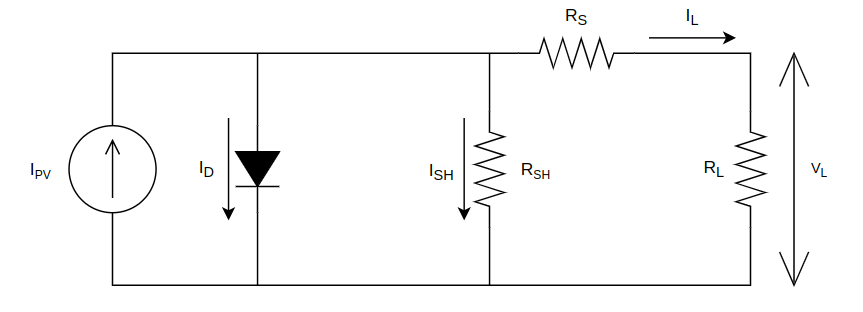
\includegraphics[width=\textwidth]{solar_cell_five_parameter_model.png}
    \caption{Five Parameter, or Full Single Diode Model of a Solar Cell}
    \label{fig:single_diode_model_with_resistances}
\end{figure}

The most common model for solar cells is the five parameter solar cell model,
shown in \autoref{fig:single_diode_model_with_resistances}. This is the complete
form of the single diode model discussed in the previous section,
\autoref{subsec:three_parameter_solar_cell_model}. There are two added
components/parameters: a \acf{RS} and \acf{RSH}, whose primary roles are to
alter the shape of the knee-bend in the I-V curve. As such, this model improves
upon the main flaw of the three parameter solar cell model, that of poorly
predicting points clustering around the maximum power point.

In the following, we discuss the two added parameters and their specific effects
on the model.


\subsubsection{Shunt Resistance}\label{subsubsec:five_param_shunt_resistance}

\begin{figure}[h]
    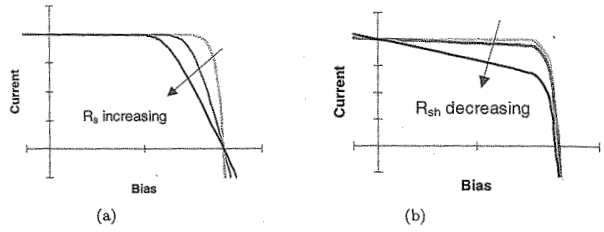
\includegraphics[width=\textwidth]{series_shunt_resistance.png}
    \caption{Effect of Series (a) and Shunt Resistance (b) on \ac{I-V} Curve}
    \label{fig:series_shunt_resistance}
\end{figure}

As shown in \autoref{fig:series_shunt_resistance} (b) from Nelson~\cite{nelson},
as the \acf{RSH} decreases, the top of the knee-bend of the \acf{I-V} curve will
be forced down. At low values of \ac{RSH} (on the order of $10$ $\si{\ohm}$),
the knee-bend will be pushed down so much that the curve becomes a straight
line. At high values of \ac{RSH}, (on the order of $100$ $\si{\ohm}$), the curve
converges to some fixed maximum bend constrained by other parameters of the
model. This relationship is generally considered logarithmic.

The \acf{ISH} can be added to the simple form of the model as a new term as
shown in \autoref{eq:cell_output_current_3}. Assuming that the \acf{RS} is
negligible ($0$), we can determine that \ac{ISH} is a function of the \ac{RSH}
and the \acf{VL}, as shown in \autoref{eq:cell_output_current_4}.

\begin{equation}
    I_L = I_{PV} - I_D - I_{SH}
    \equnit{\si{\ampere}}
    \label{eq:cell_output_current_3}
\end{equation}

\begin{equation}
    I_L = I_{PV} - I_D - \frac{V_L}{R_{SH}}
    \equnit{\si{\ampere}}
    \label{eq:cell_output_current_4}
\end{equation}


\subsubsection{Series Resistance}\label{subsubsec:five_param_series_resistance}

The \acf{RS} forces the knee-bend of the \ac{I-V} curve to the left or right, as
opposed to up and down for \ac{RSH}. As \ac{RS} increases, more current is
consumed across the lumped resistance before reaching the terminals of the solar
cell, reducing the expected current in the curve as shown in
\autoref{fig:series_shunt_resistance} (a). At high values of \ac{RS}, the curve
likewise becomes a straight line.

The \ac{RS} term impacts the consumers of the five parameter solar cell model;
namely the \ac{ID} and the \ac{RSH} terms. A visualization of this is shown as
\autoref{fig:current_junction}.

\begin{figure}[!htbp]
    \centering
    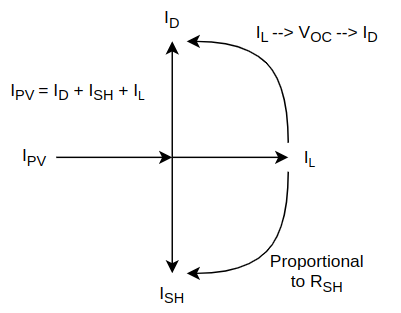
\includegraphics[width=0.6\textwidth]{cell_kirchoff_current_junction.png}
    \caption{Current Flow Junction of Five Parameter Model Solar Cell}
    \label{fig:current_junction}
\end{figure}

Revisiting \autoref{eq:cell_dark_current_1}, we know that the dark current
depends on \acf{VL} generated by \acf{IL} flowing through equivalent \acf{RL} connected at the cell
terminals. This allows us to reformulate the dark current equation as
\autoref{eq:cell_dark_current_2}. Here, we add the voltage drop across the
lumped series resistance summed with the \ac{VL} to represent the
total voltage expected by the dark current model.

\begin{equation}
    I_D = I_0[\exp(\frac{V_L + I_L R_S}{V_T}) - 1]
    \equnit{\si{\ampere}}
    \label{eq:cell_dark_current_2}
\end{equation}

We can likewise use the voltage drop to update the \ac{ISH} term, shown
in \autoref{eq:cell_shunt_current}.

\begin{equation}
    I_{SH} = \frac{V_L + I_L R_S}{R_{SH}}
    \equnit{\si{\ampere}}
    \label{eq:cell_shunt_current}
\end{equation}

Combining these two effects, we form \autoref{eq:cell_output_current_5}.

\begin{equation}
    I_{L} =  I_{PV} - I_0[\exp(\frac{V_L + I_L R_S}{V_T}) - 1] - \frac{V_L + I_L R_S}{R_{SH}}
    \equnit{\si{\ampere}}
    \label{eq:cell_output_current_5}
\end{equation}

We note that this model is an implicit function and cannot easily (or prettily)
move all the \ac{IL} terms to the left side of the equation. As such, for these
types of problems, we will develop and use iterative solvers to determine
\ac{IL} for a given set of input parameters (\ac{RS}, \ac{G}, \ac{VL}, etc).
Iterative solvers involve starting with a guess for the output parameter (in
this case \ac{IL}) and attempt to improve upon that guess such that each side is
equal to each other or within some tolerance to each other. An in depth
discussion on how these solvers were implemented for this model and variants of
this model can be found in \autoref{appendix:iterative_solvers}.

\todo[inline]{Augment appendix note with reference to
\ref{subsubsec:modeling_solar_cell_datasets}. Relegate appendix note to discussion
about iterative solvers and steps to build iterative solver (Desmos -\> MATLAB -\>
Python).}


\subsubsection{Photocurrent as a Ratio of Shunt/Series Resistance}\label{subsubsec:photocurrent_shunt_series_relation}

An interesting addition to the five parameter cell model is presented by Cubas
et al~\cites{cubas_et_al,cubas_et_al_2}: they observe that
\autoref{eq:cell_output_current_5} in short circuit conditions results in
\autoref{eq:cell_short_circuit_current_6}.

\begin{equation}
    I_{SC} = I_{PV} - I_0[\exp(\frac{I_{SC} R_S}{V_T}) - 1] - \frac{I_{SC} R_S}{R_{SH}}
    \equnit{\si{\ampere}}
    \label{eq:cell_short_circuit_current_6}
\end{equation}

In their analysis of measurements taken across a broad spectrum of reference
solar cells, represented in \autoref{table:dark_current_reference}, the dark
current at short circuit conditions were well less than a single milliampere, an
insignificant fraction of the total operating current. From this observation
Cubas et al. rewrites the above expression to get the photocurrent as a function
of \ac{ISC} and a ratio of \ac{RS} and \ac{RSH}, shown in
\autoref{eq:cell_photocurrent_3}.

\begin{equation}
    I_{PV} = I_{SC}\frac{R_S + R_{SH}}{R_{SH}}
    \equnit{\si{\ampere}}
    \label{eq:cell_photocurrent_3}
\end{equation}

\begin{table}[h!]
    \begin{tabularx}{\textwidth}{
        | >{\raggedright\arraybackslash}X
        | >{\raggedright\arraybackslash}X
        | >{\raggedright\arraybackslash}X
        | >{\raggedright\arraybackslash}X
        | >{\raggedright\arraybackslash}X | }
        \hline
        Reference & Cell Type & \ac{ISC} (A) & $I_0[e^{\frac{I_{SC} R_S}{V_T}} -
        1]$ (A) & \ac{ID} / \ac{ISC} \\ \hline \hline
        Kennerud, 1969  & CdS   & 0.8040 & 1.56E-5 & 1.94E-5 \\ \hline
        Charles, 1981   & BSC   & 0.1023 & 2.21E-8 & 2.16E-7 \\ \hline
        Charles, 1981   & GSC   & 0.5610 & 1.01E-5 & 1.80E-5 \\ \hline
        Lo Brano, 2010  & Q6LM  & 7.6650 & 1.42E-9 & 1.85E-10 \\ \hline
    \end{tabularx}
    \caption{Dark Current Ratios for Various Reference Cells~\cite{cubas_et_al}}
    \label{table:dark_current_reference}
\end{table}

However, a cursory evaluation of the parameter space (\ac{VOC}, \ac{ISC},
\ac{G}, \ac{TC}, \ac{RS}, \ac{N}) reveals that the assumption that the dark
current is negligible breaks down when a subset of the following conditions
occur:

\begin{itemize}
    \item the \acf{VOC} becomes very small,
    \item the \acf{ISC} becomes very large,
    \item and the \acf{RS} becomes relatively large for some
    combination of \ac{VOC} and \ac{ISC}.
\end{itemize}

Is it to be noted that these parameters are tightly coupled, and therefore the
language specifying a parameter space upon which this term should be used
remains imprecise. We also note that \ac{TC} and \ac{N} when increased slightly
tighten the viable parameter space.

However, when considering a specific solar cell that is \textit{appropriate}
(e.g.\ it contains \ac{STC} defined parameters \ac{VOC} and \ac{ISC} with an
measured \ac{RS} that results in negligible \ac{ID}), this term remains
negligible unless the cell is exposed to (1) high temperatures or (2) high
intensity light, two conditions that tend to come hand in hand. These conditions
tend to only be experienced by concentrator photovoltaics and are highly
unlikely to be reached by normal solar cells.

We will observe later in \autoref{subsec:eval_solar_cell_models} that with our
dataset of Maxeon Gen III Bin Le1 solar cells, the vast majority of estimated
series resistance is well below $0.08 \si{\ohm}$, which results in dark currents
less than a m\si{\ampere}. This means that this modification (assuming it
improves the accuracy of the model), is well suited for our solar cells.

Incorporating this revision, we arrive at
\autoref{eq:cell_short_circuit_current_7}.

\begin{equation}
    I_L = I_{SC}\frac{R_S + R_{SH}}{R_{SH}} - I_0[\exp(\frac{V_L + I_L R_S}{V_T}) - 1] - \frac{V_L + I_L R_S}{R_{SH}}
    \equnit{\si{\ampere}}
    \label{eq:cell_short_circuit_current_7}
\end{equation}

\todo[inline]{See \url{https://www.desmos.com/calculator/nniw0mha2k} to play
around with the revised dark current model. Add as a figure later on compared to
experimental data.}


\subsubsection{Shunt and Series Resistance as a Function of Irradiance, Temperature}\label{subsubsec:rsh_rs_dependence}

Throughout this discussion, we introduced the notion of shunt and series
resistance as internal parasitics. However, we did not explore whether these
`internal parameters' are themselves affected by external conditions such as
irradiance and temperature.

A comprehensive review and experimental paper from Fébba et
al~\cite{febba_et_al} performed experiments on solar cells to evaluate the
effect of temperature and irradiance on shunt and series resistance, controlling
for the two independent variables in ranges of $25\si{\celsius}$ to
$55\si{\celsius}$ and $600\si{\watt/\meter^2}$ to $1000\si{\watt/\meter^2}$,
respectively. Four figures,
\autoref{fig:febba_shunt_resistance_and_temperature}~-~\autoref{fig:febba_series_resistance_and_irradiance}
are shown below to illustrate the following assertions.

For \acf{RSH}, they observed the following trends:

\begin{itemize}
    \item as temperature increases, the \ac{RSH} exponentially decays,
    \item and as irradiance increases, the \ac{RSH} linearly decreases.
\end{itemize}

For \ac{RS}, they observed the following trends:

\begin{itemize}
    \item as temperature increases, the \ac{RS} exponentially decays,
    \item and as irradiance increases, the \ac{RS} linearly increases.
\end{itemize}

\begin{figure}[!htbp]
    \centering
    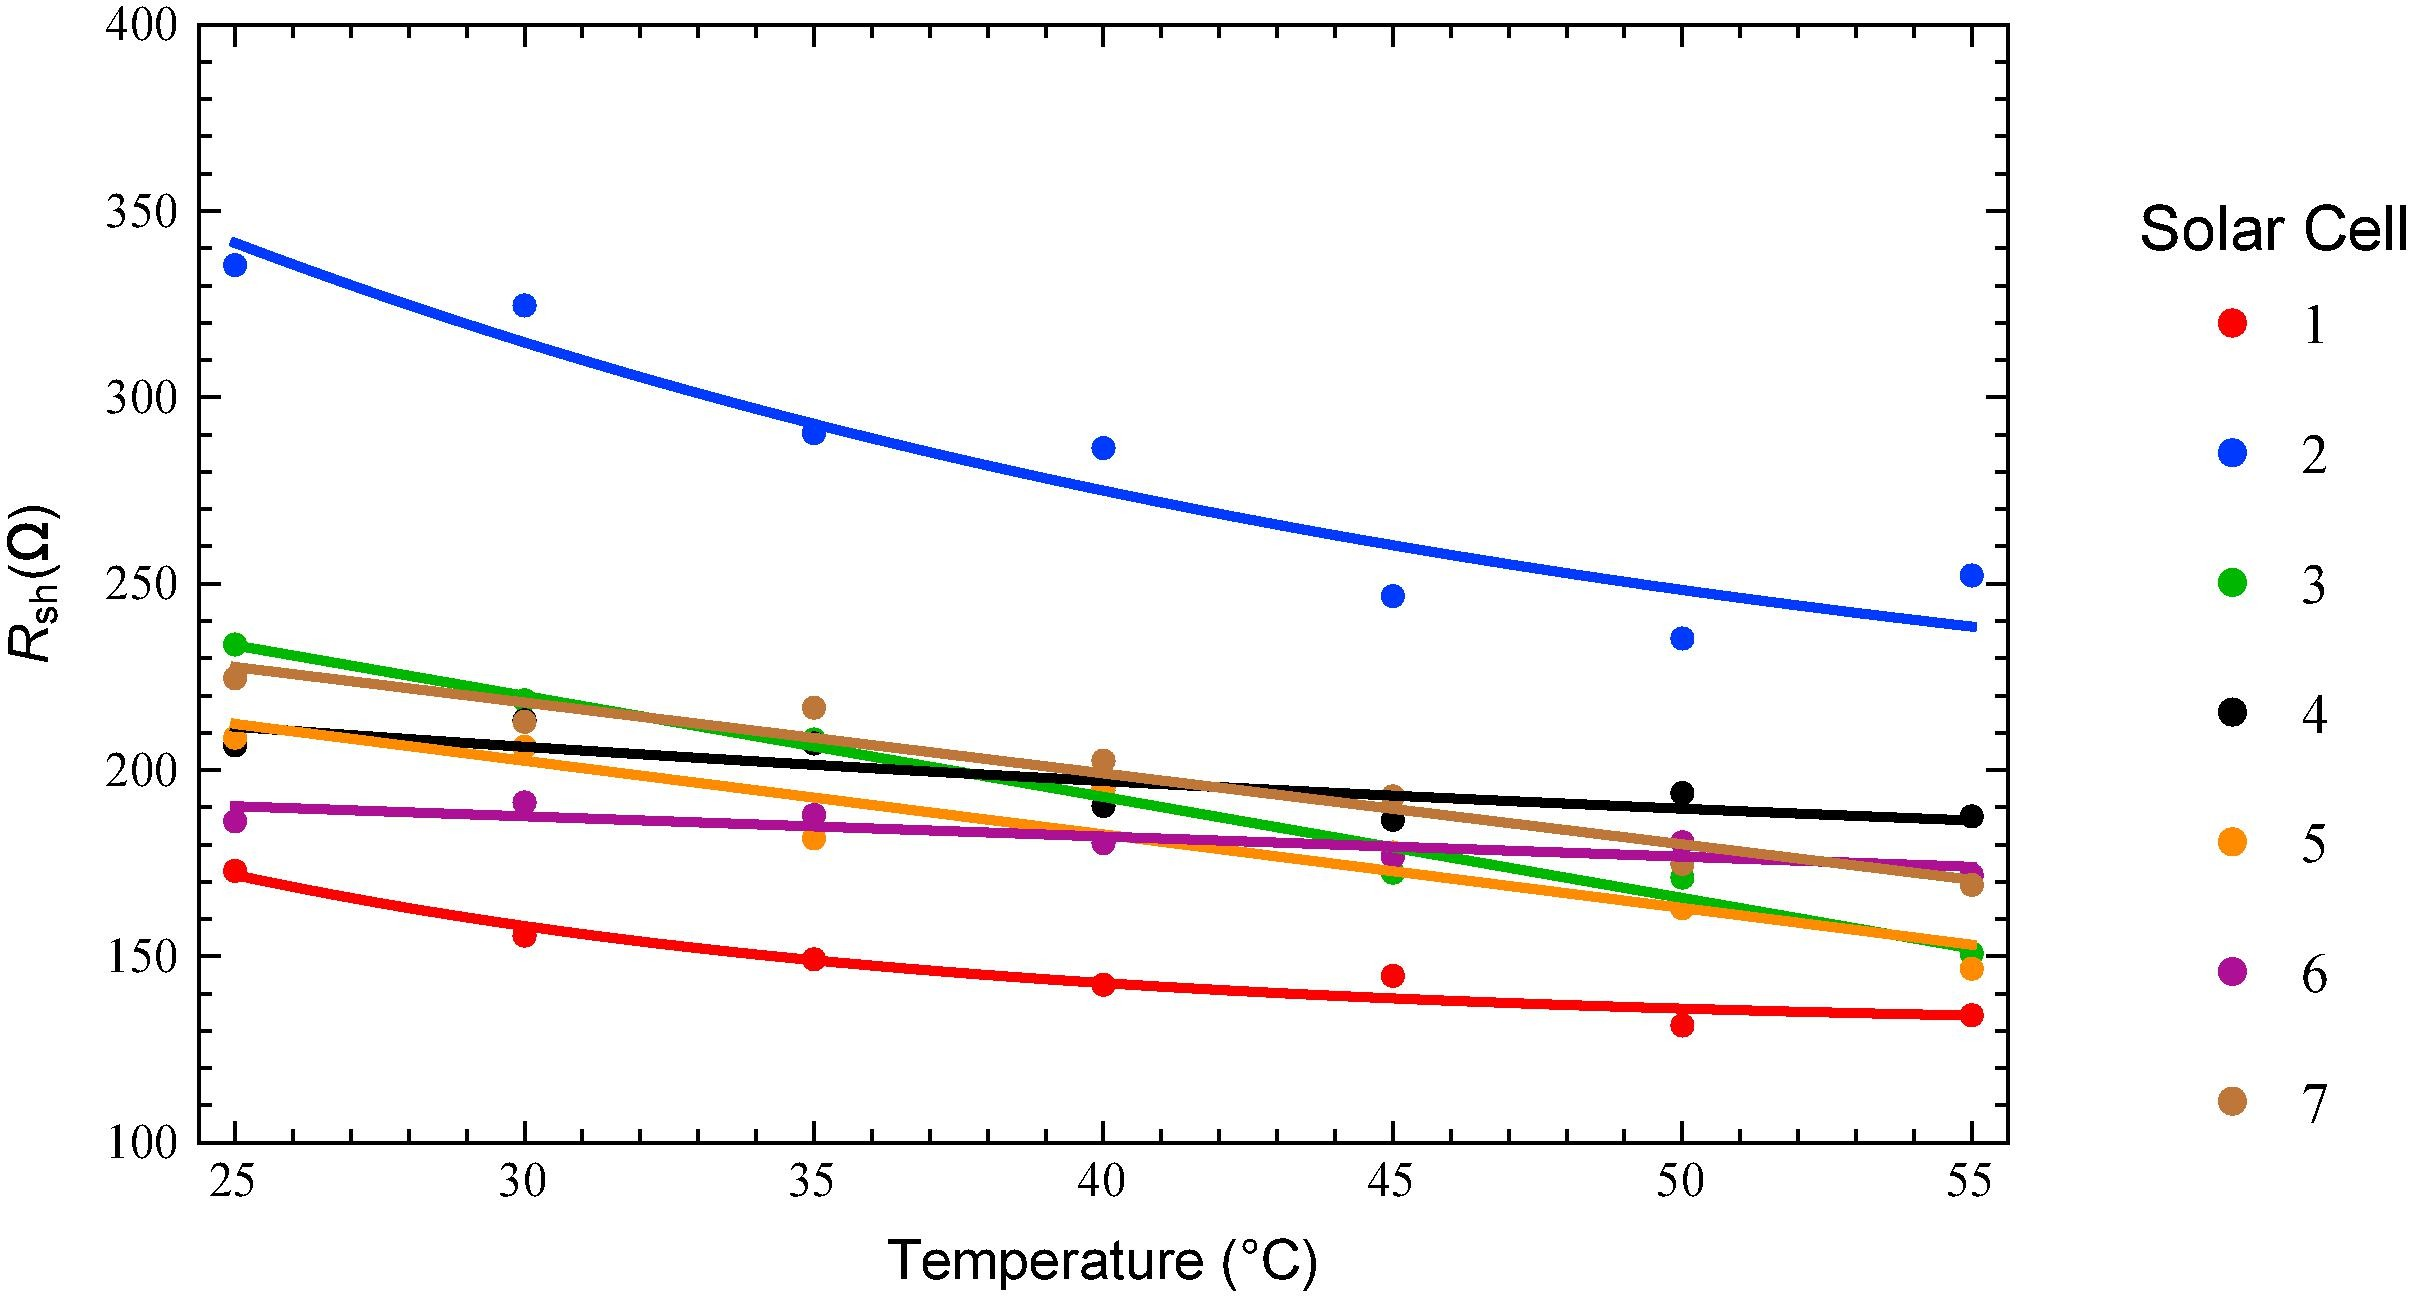
\includegraphics[width=\textwidth]{febba_shunt_resistance_and_temperature.jpg}
    \caption{Shunt Resistance vs Temperature~\cite{febba_et_al}}
    \label{fig:febba_shunt_resistance_and_temperature}
\end{figure}

\begin{figure}[!htbp]
    \centering
    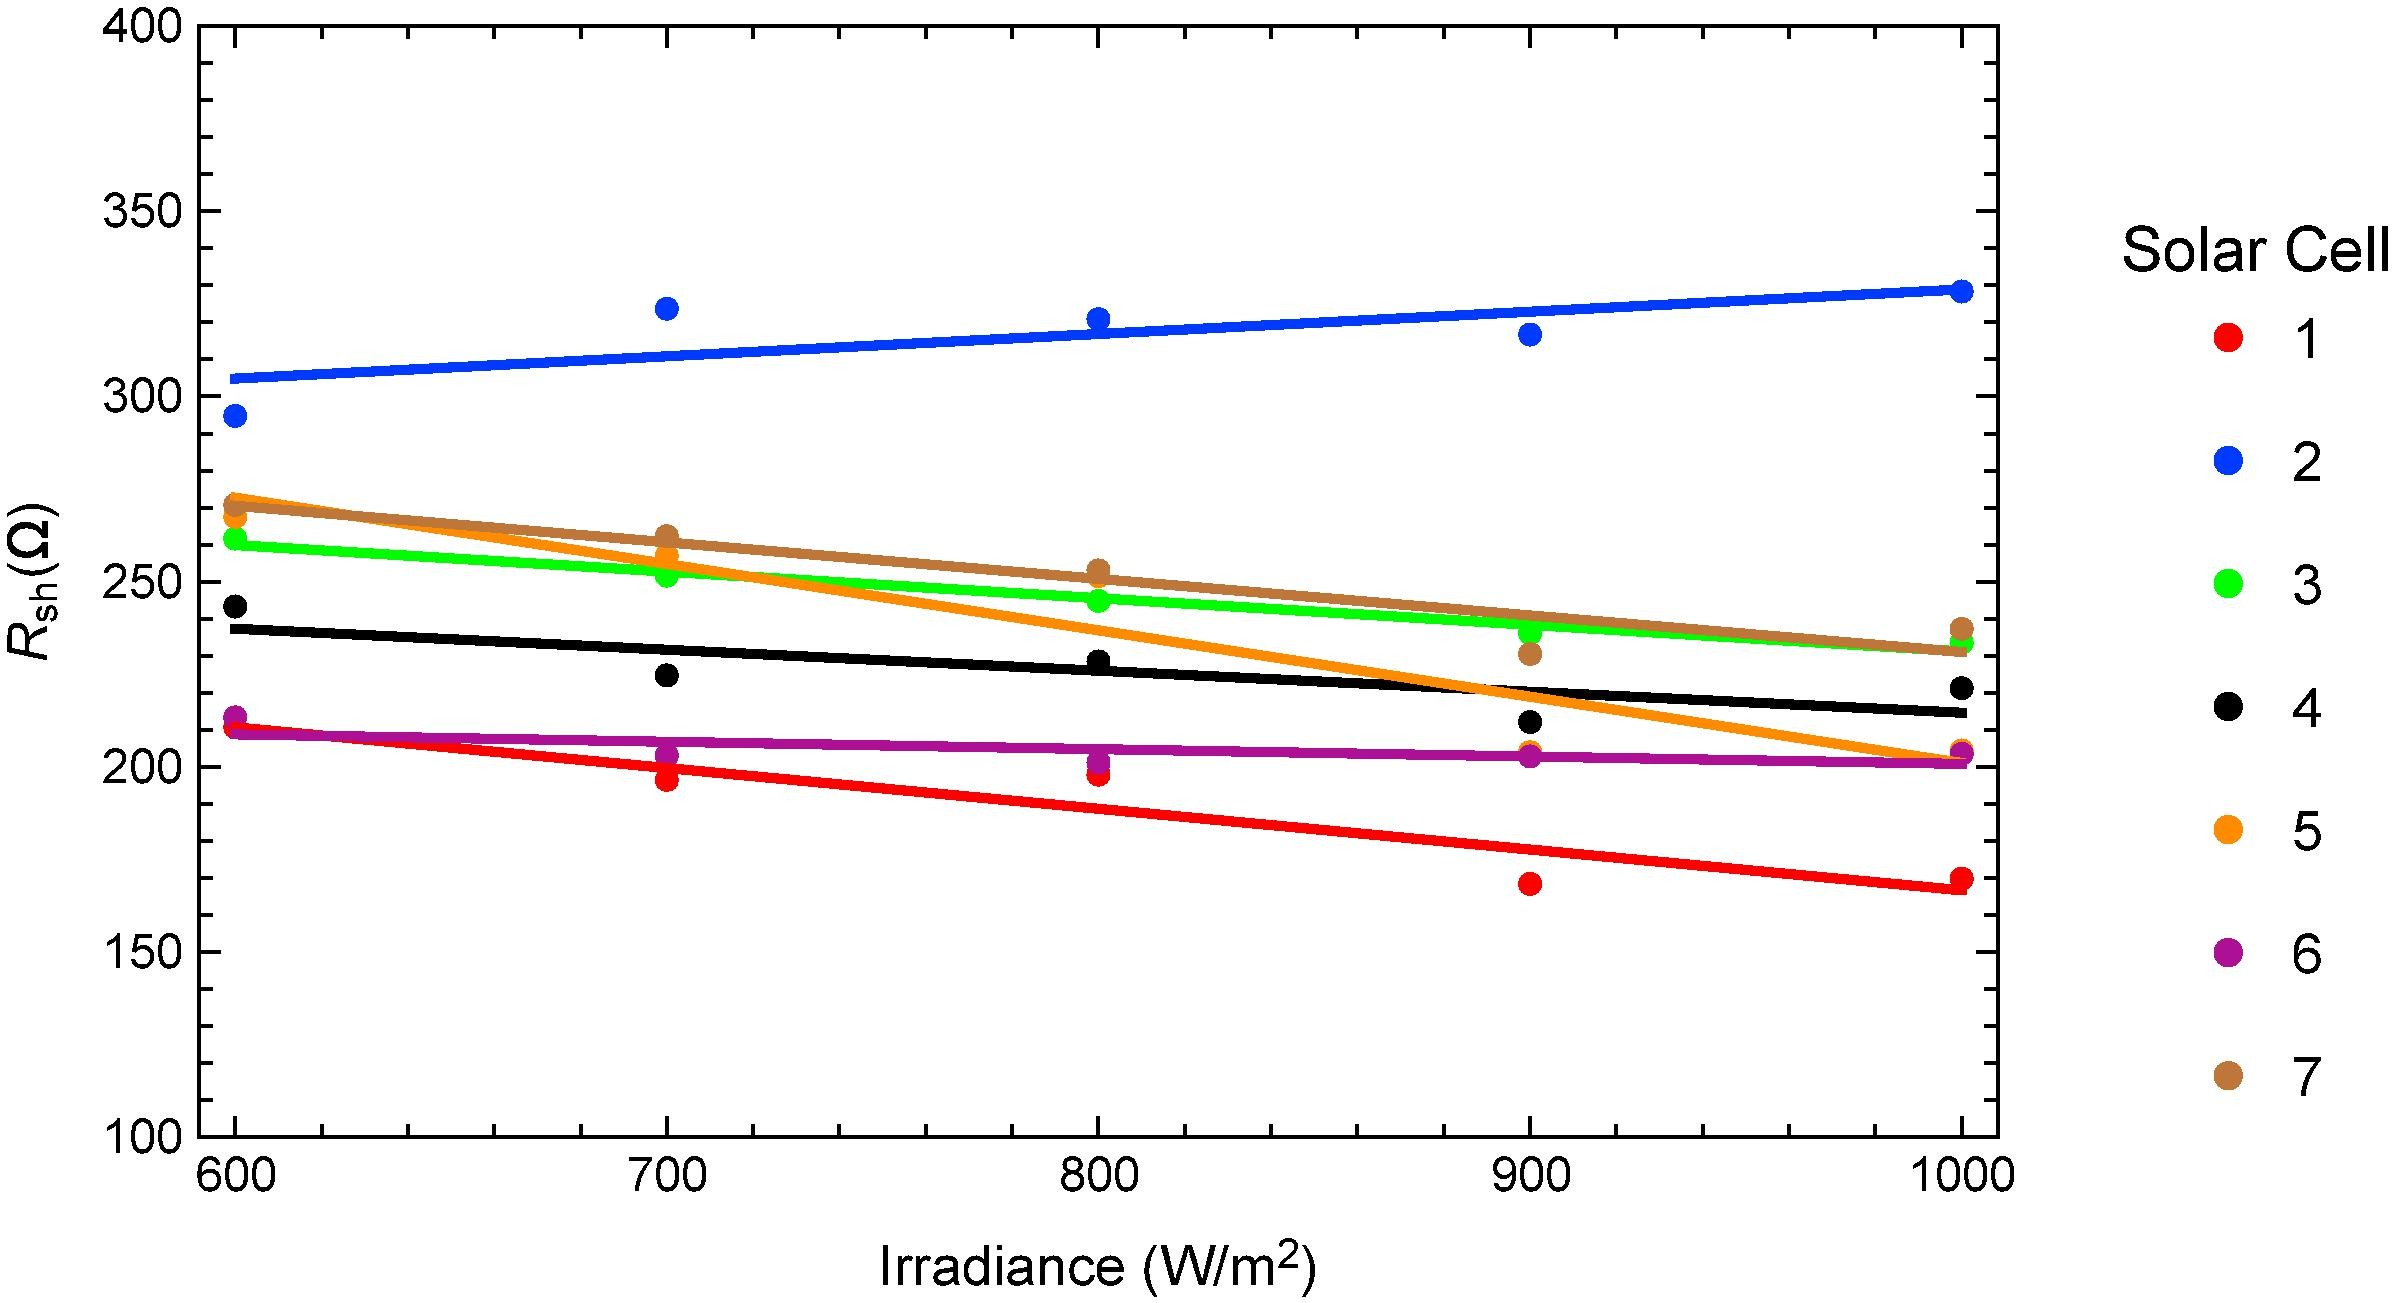
\includegraphics[width=\textwidth]{febba_shunt_resistance_and_irradiance.jpg}
    \caption{Shunt Resistance vs Irradiance~\cite{febba_et_al}}
    \label{fig:febba_shunt_resistance_and_irradiance}
\end{figure}

\begin{figure}[!htbp]
    \centering
    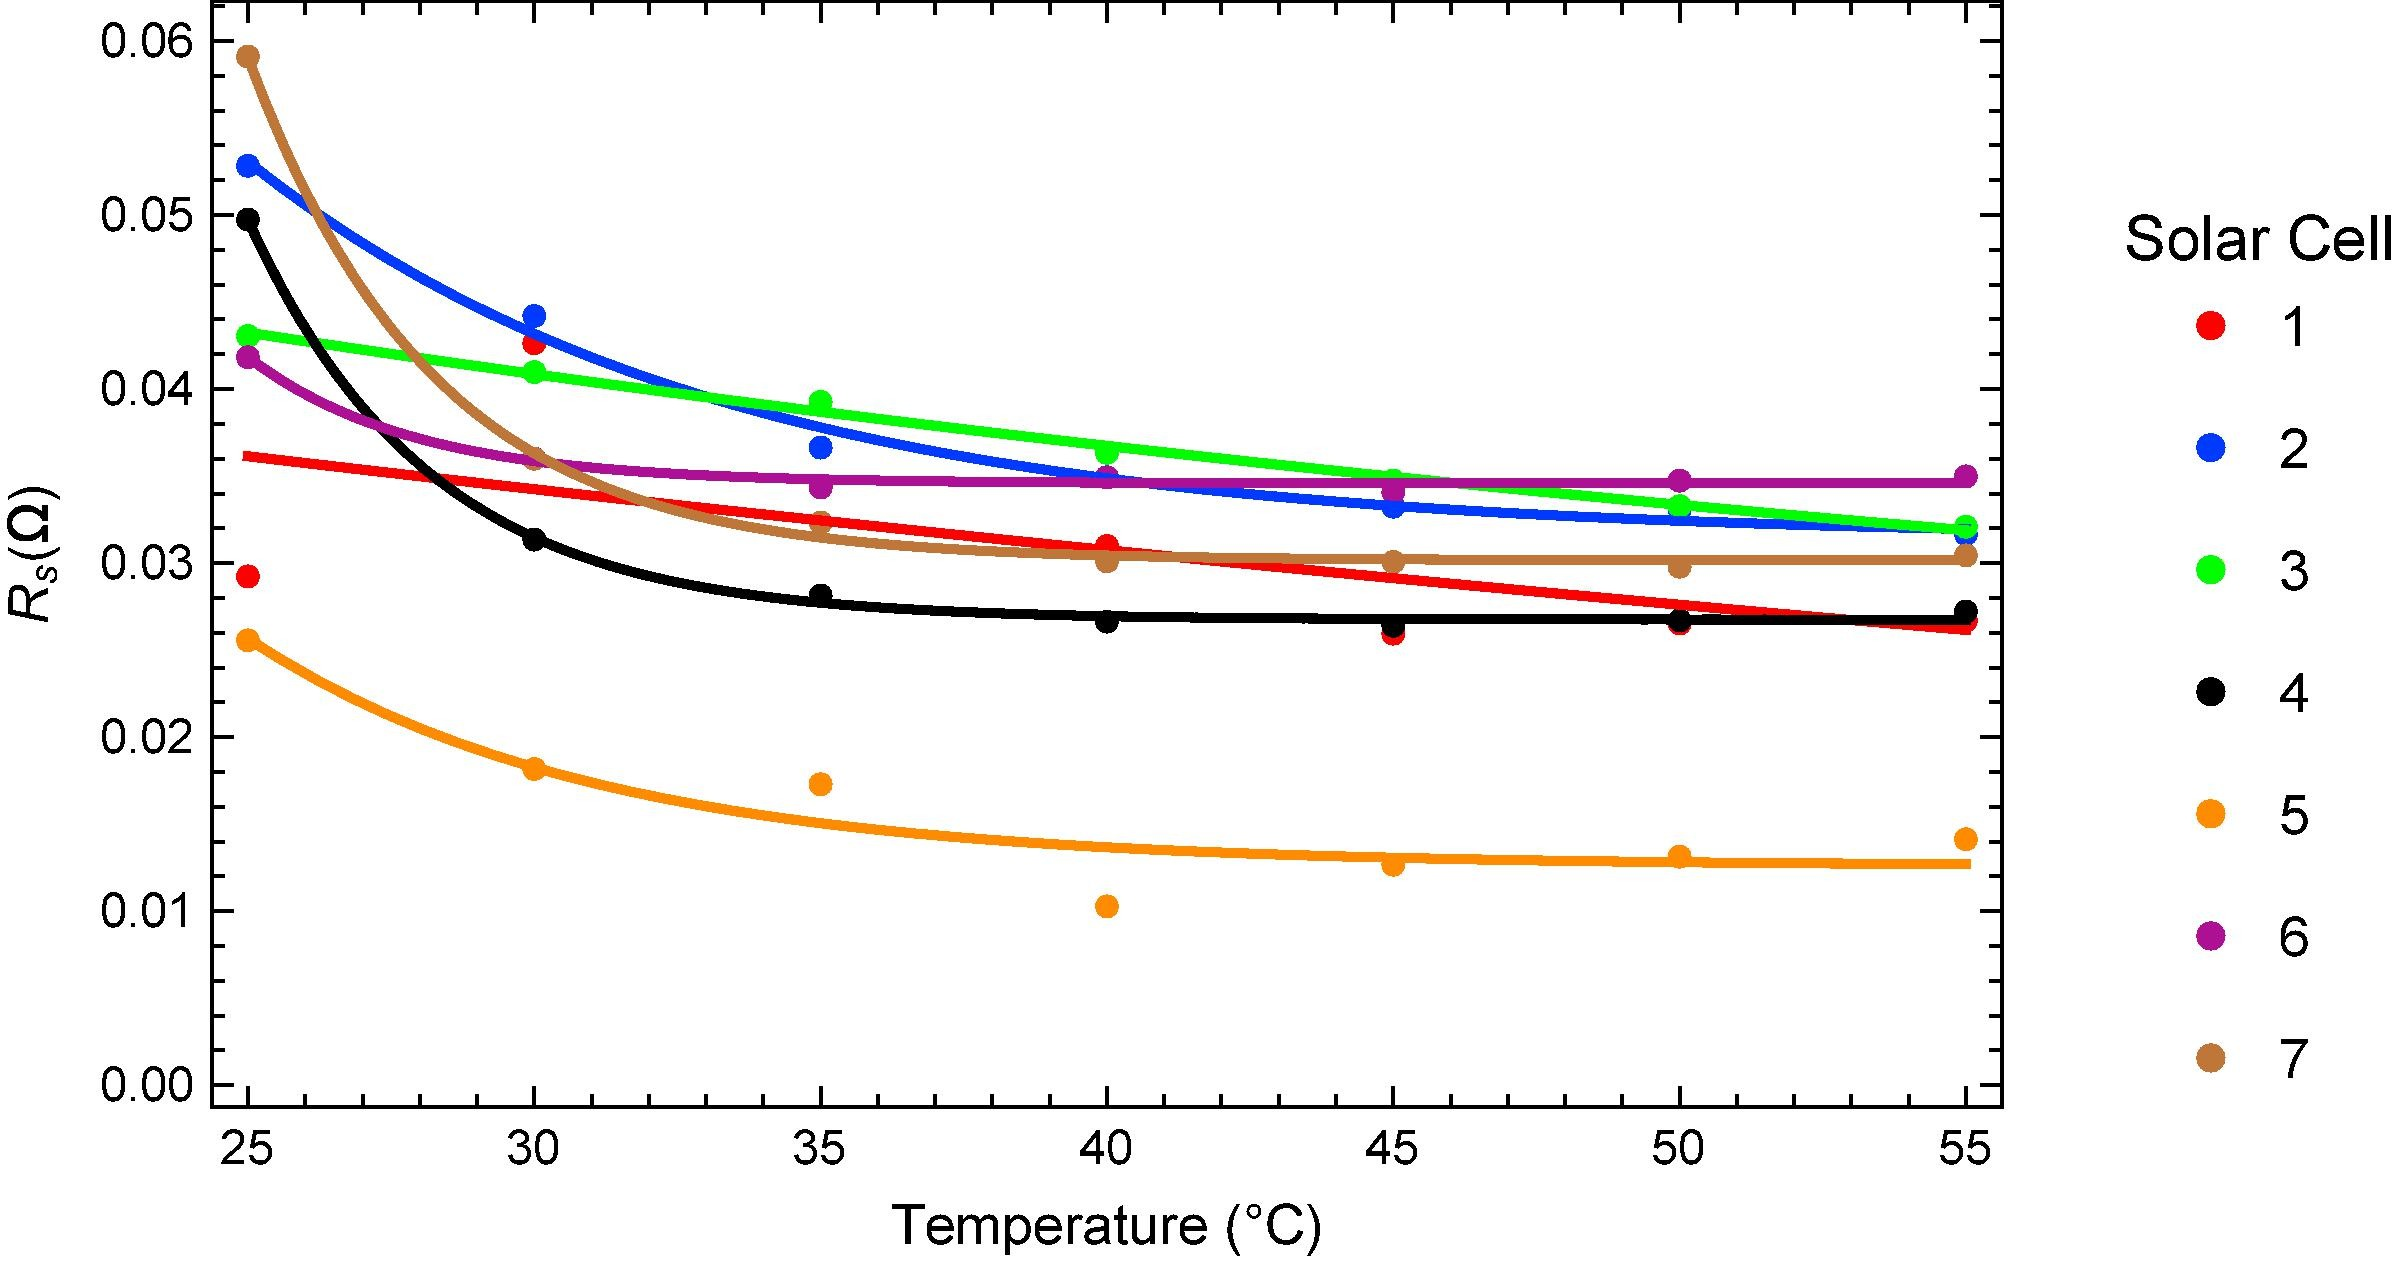
\includegraphics[width=\textwidth]{febba_series_resistance_and_temperature.jpg}
    \caption{Series Resistance vs Temperature~\cite{febba_et_al}}
    \label{fig:febba_series_resistance_and_temperature}
\end{figure}

\begin{figure}[!htbp]
    \centering
    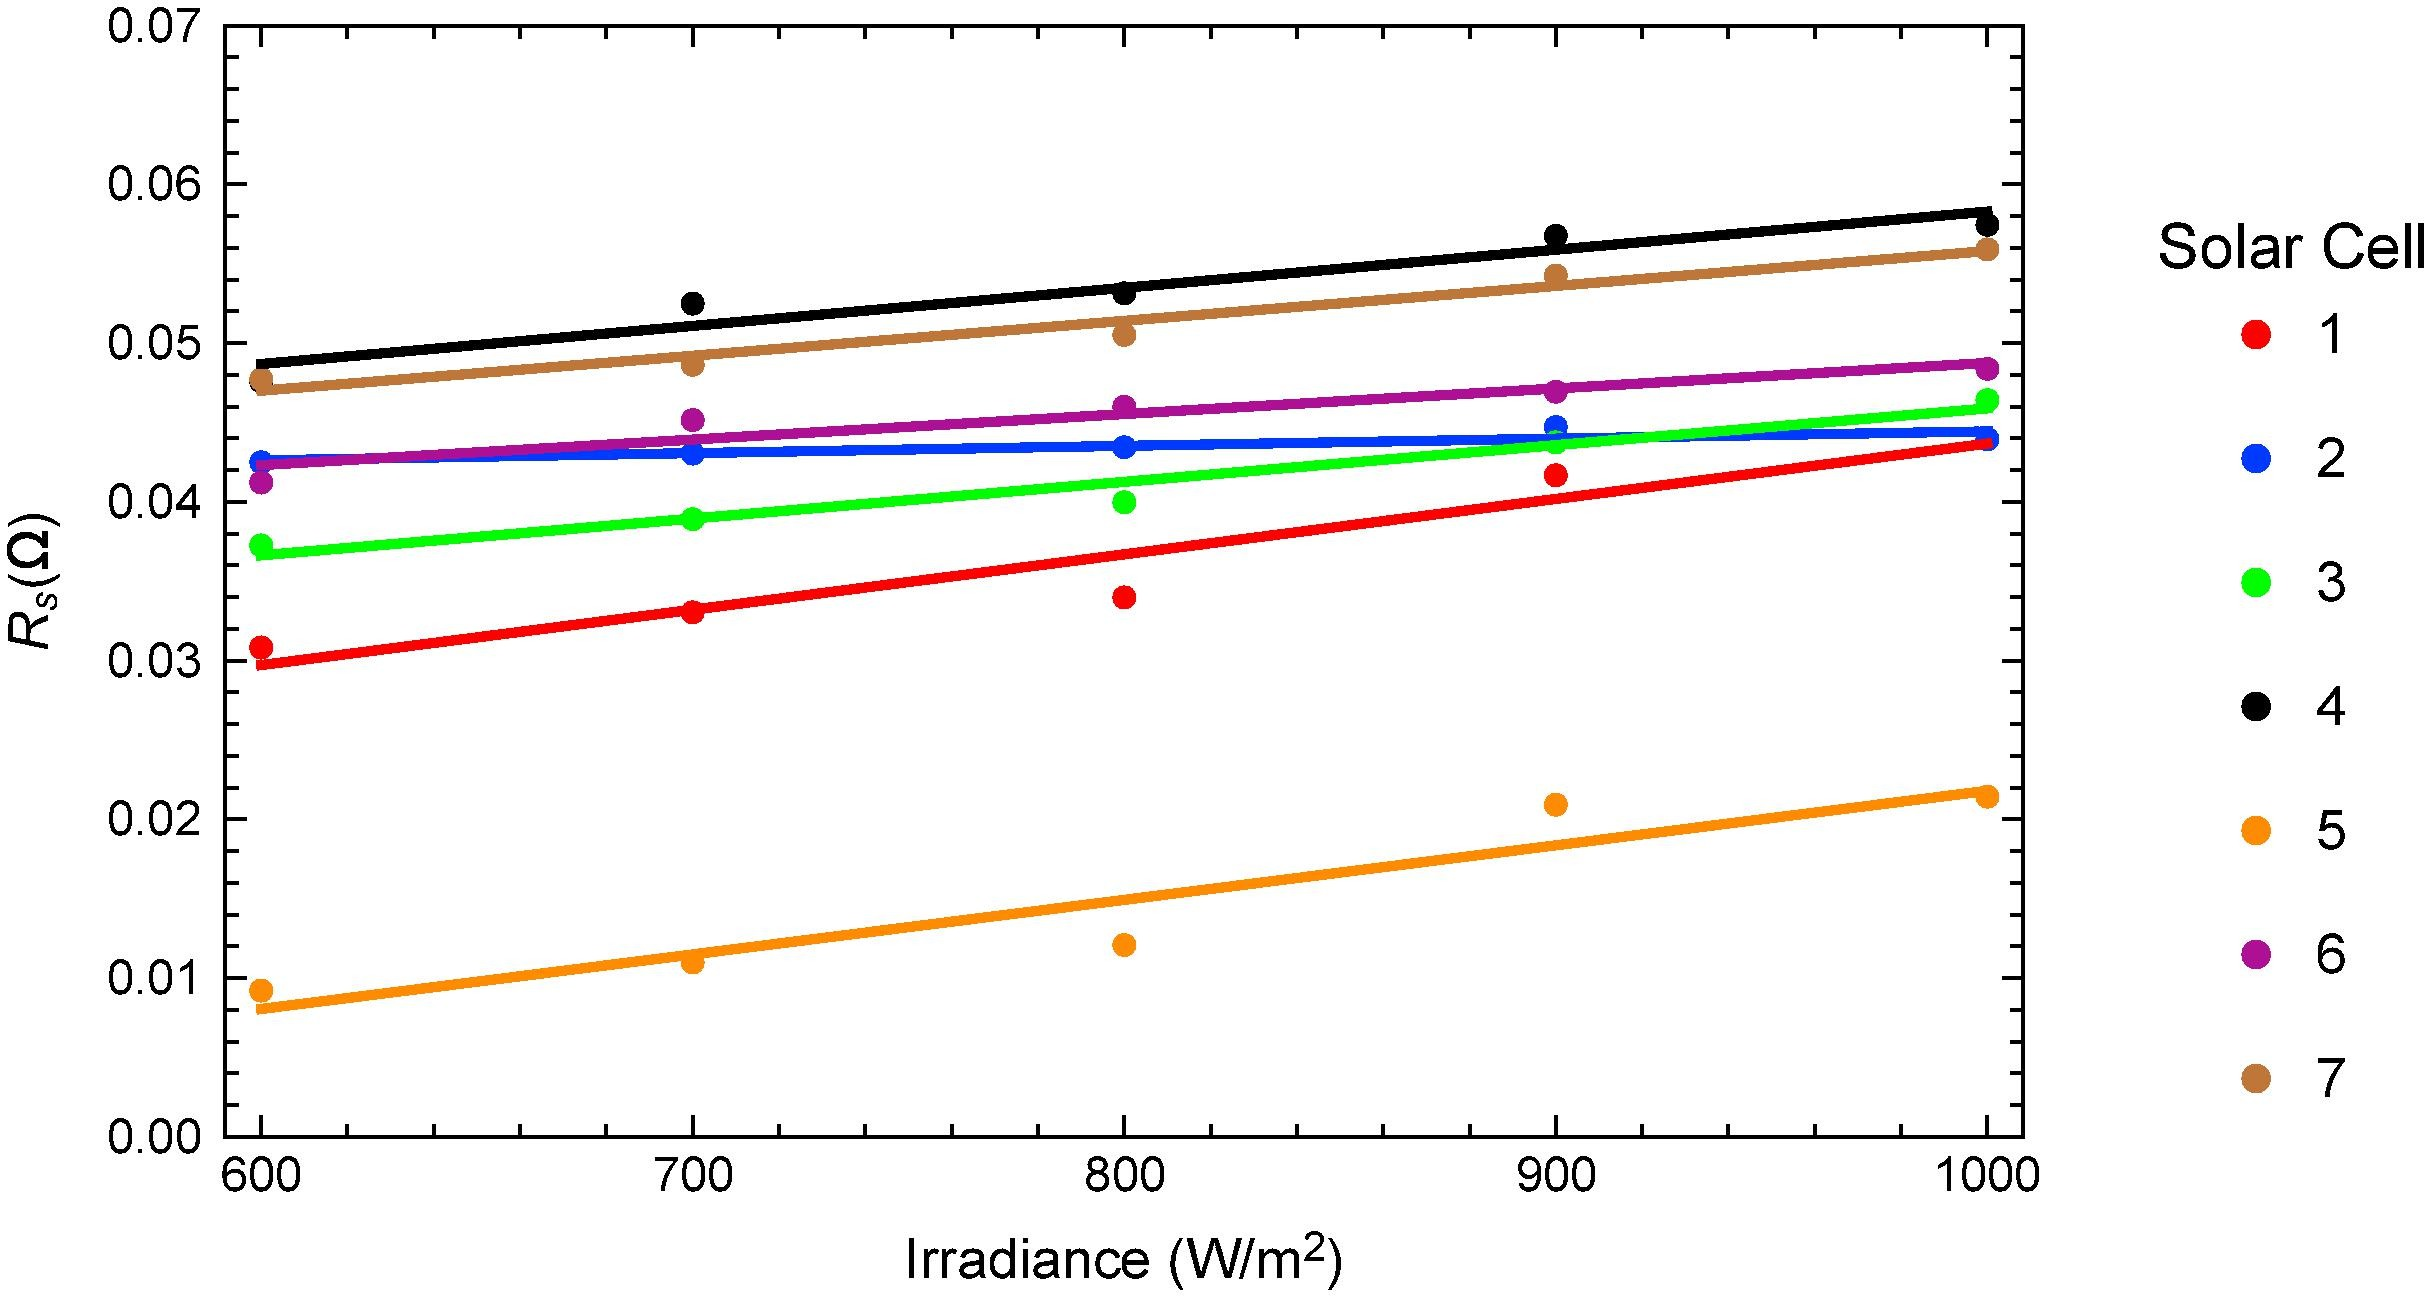
\includegraphics[width=\textwidth]{febba_series_resistance_and_irradiance.jpg}
    \caption{Series Resistance vs Irradiance~\cite{febba_et_al}}
    \label{fig:febba_series_resistance_and_irradiance}
\end{figure}

Fébba et al. did not posit a revised model of the either resistance term
(although they did provide explanations on why the trends were reasonable), but
Baig et al.~\cite{baig_et_al} and MacAlpine et
Brandemuehl~\cite{macalpine_et_brandemuehl} introduced a variant of
\autoref{eq:series_resistance_1} that uses a \ac{ZETA}.

\begin{equation}
    R_S = R_{S,ref} \exp(\zeta [T_{C,ref} - T_C])
    \equnit{\si{\ohm}}
    \label{eq:series_resistance_1}
\end{equation}

We extend Fébba et al~\cite{febba_et_al}'s results to generate
\autoref{eq:series_resistance_2}, adding a \ac{ETA}, applied to
\autoref{eq:series_resistance_1}.

\begin{equation}
    R_S = R_{S,ref} \exp(\zeta [T_{C,ref} - T_C])[1 + \eta(G_{ref} - G)]
    \equnit{\si{\ohm}}
    \label{eq:series_resistance_2}
\end{equation}

We also propose \autoref{eq:shunt_resistance} to model the shunt
resistance, with \ac{KAPPA} and \ac{IOTA}.

\begin{equation}
    R_{SH} = R_{SH,ref} \exp(\kappa [T_{C,ref} - T_C])[1 + \iota [G_{ref} - G]]
    \equnit{\si{\ohm}}
    \label{eq:shunt_resistance}
\end{equation}

\autoref{eq:series_resistance_2} and \autoref{eq:shunt_resistance}'s
coefficients are not provided by the manufacturer, so they will have to be
estimated. We'll look at ways to measure series and shunt resistance in
\autoref{subsubsec:experimental_extraction_of_cell_parameters}, and how to take
advantage of our test setup to measure the coefficients. Additionally, we'll
attempt to replicate Fébba et al's work on a broader scale, with a temperature
and irradiance range of ($0\si{\celsius}$ to $100\si{\celsius}$
and $0\si{\watt/\meter^2}$ to $1000\si{\watt/\meter^2}$, respectively).


\subsubsection{Non Uniform Series Resistance}\label{subsubsec:nonuniform_series_resistance}

As an aside to this thesis, we note that the solar cell models described assume
that the cell is uniform in composition and thus can represent the series
resistance as a lumped resistance. In actuality, the cell is a two (actually
three, but for all intents and purposes the thickness is irrelevant in terms of
affecting the series resistance -although it may affect the shunt resistance)
dimensional network of resistors and diodes
(\autoref{fig:cell_with_varying_series_resistance}).

\begin{figure}[!htbp]
    \centering
    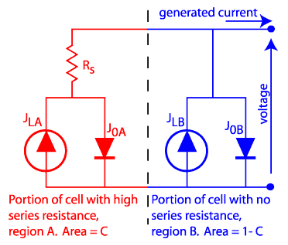
\includegraphics[width=0.6\textwidth]{cell_with_varying_series_resistance.png}
    \caption{Solar Cell With Varying Series Resistances~\cite{pveducation_measurement_of_series_resistance}}
    \label{fig:cell_with_varying_series_resistance}
\end{figure}

If the cell series resistance was measured using two probes at various points in
the cell, we would likely see that the places of smallest resistance will focus
on the direct paths between two terminals; the places of largest resistance will
be at the edges of the cell where the current path is longest. This is
visualized on a Maxeon Gen III cell in
\autoref{fig:maxeon_gen_iii_cell_current_resistance_path}, where the darker
paths represent higher resistances.

\begin{figure}[!h]
    \centering
    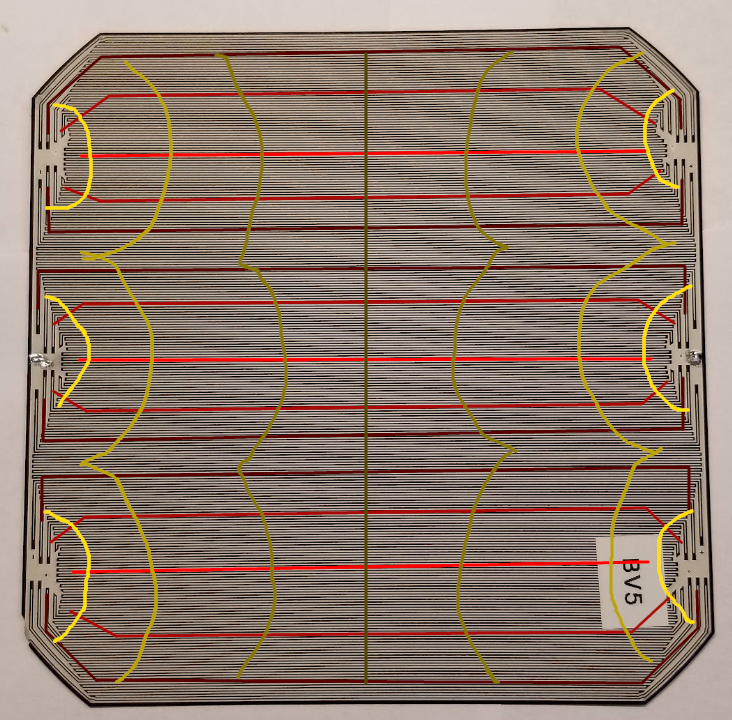
\includegraphics[width=0.88\textwidth]{maxeon_gen_iii_cell_current_resistance_paths.png}
    \caption{Current Paths of Maxeon Gen III Cell}
    \label{fig:maxeon_gen_iii_cell_current_resistance_path}
\end{figure}

This series resistance non uniformity becomes more important to the
resultant \ac{I-V} curve in low light conditions. Under uniform, bright
conditions, current from the photovoltaic effect is generated evenly and
conducts to the contacts regardless of the resistance along the paths. In the
dark, any current that has to flow through the cell (either from a partially
unshaded region or from an external source) will favor the shortest/least
resistive paths. As such, we would expect the apparent series resistance to vary
in various lighting contexts.

For the purposes of this thesis, we will continue to assume that the solar cell,
the base unit of our model, is uniform in internal and external characteristics.
However, we will look at intercell variance in our module models. Further
research into intracell series variance is explored by Bowden et
Rohatgi~\cite{bowden_et_rohatgi}.


\subsubsection{Model Summary}\label{subsubsec:five_param_model_summary}

To conclude this discussion, we will review the components that make up the
five parameter cell model, propose an item of further exploration, and propose a
complete model function that incorporates the topics discussed.

Firstly, the five parameter cell model retains the attributes of the three
parameter cell model, being the complete form of the single diode model. It adds
two parameters, a \acf{RSH} and \acf{RS} that represent ohmic losses in the
solar cell, which primarily affect the knee-bend of the resultant \ac{I-V}
curve. These two parameters help reduce error in the model around the knee-bend
that cannot fully be represented by the ideality factor. However, these
additions increase the complexity of the model, and the resultant form is an
implicit equation that requires an iterative solver approach.

Secondly, we investigate a revision to the photocurrent model to make it also a
function of \ac{RS} and \ac{RSH}. This was obtained by evaluating the short
circuit condition of the existing model and reducing the dark current term under
appropriate conditions. We note that this new model may not work under specific
conditions, namely for concentrator solar cells or for solar cells with
inordinately large series resistance relative to their specific \ac{VOC} and
\ac{ISC} combination.

We also discuss evaluating \ac{RS} and \ac{RSH} themselves as a function of
temperature and irradiance. We observe that these values tend to have
exponential relationships with temperature and linear relationships with
irradiance, although we require further data to validate the strength of these
correlations. We derive initial models for these parameters, and discuss real
world conditions in which they might deviate from our expectations (e.g. partial
shading). As such, we will revisit both of these modifications to the base model
in a further discussion to prove or disprove their veracity and usefulness to
the overall model.

Finally, we incorporate these changes into the complete function defined in the
previous sections. This is presented as \autoref{eq:cell_output_current_6}
(\ac{ISC}, \ac{VOC}, \ac{RS}, \ac{RSH}, and \ac{VT} abstracted out for clarity
and brevity). We observe that this complete model builds upon the existing
parameters named in \autoref{subsubsec:three_param_model_summary} by adding two
extra reference parameters:

\begin{itemize}
    \item \acf{RSREF}
    \item \acf{RSHREF}
\end{itemize}

and four more curve fitting parameters:

\begin{itemize}
    \item \acf{ZETA}
    \item \acf{ETA}
    \item \acf{KAPPA}
    \item \acf{IOTA}
\end{itemize}

Likewise with the \acf{N} and \acf{GAMMA} discussed in the three parameter solar
cell model, we will look at estimating the four new curve fitting parameters
using curve fitting and other statistical techniques. We can potentially
establish known thermal coefficients (with some error) for these cells using the
\ac{CLT}, and customize each cell with only the following variables: \ac{RSREF},
\ac{RSHREF}, which can be determined empirically using a single measurement at
\ac{STC}.


\begin{equation}
    \begin{split}
        I_L(V_L, G, T_C) &= I_{PV}(G, T_C, R_S, R_{SH}) - I_D(V_L, G, T_C, R_S) - I_{SH}(R_S, R_{SH}) \\
        & = I_{SC}(G, T_C)\frac{R_S + R_{SH}}{R_{SH}} - I_0(G, T_C)[\exp(\frac{V_L + I_L R_S}{V_T(T_C)}) - 1] - \frac{V_L + I_L R_S}{R_{SH}} \\
        & = I_{SC}(G, T_C)\frac{R_S + R_{SH}}{R_{SH}} - I_{SC}(G, T_C)\frac{\exp(\frac{V_L + I_L R_S}{V_T(T_C)}) - 1}{\exp(\frac{V_{OC}(G, T_C)}{V_T(T_C)}) - 1} - \frac{V_L + I_L R_S}{R_{SH}} \\
        & = I_{SC}(G, T_C)[\frac{R_S + R_{SH}}{R_{SH}} + \frac{1 - \exp(\frac{V_L + I_L R_S}{V_T(T_C)})}{1 - \exp(\frac{V_{OC}(G, T_C)}{V_T(T_C)})}] - \frac{V_L + I_L R_S}{R_{SH}}
    \end{split}
    \equnit{\si{\ampere}}
    \label{eq:cell_output_current_6}
\end{equation}

\todo[inline]{See \url{https://www.desmos.com/calculator/yp0rhmabkz} to play
around with the complete five parameter solar cell model. Add as a figure later
on compared to experimental data.}

\newpage
\subsection{Seven Parameter Solar Cell Model}\label{subsec:seven_parameter_solar_cell_model}

\begin{figure}[h]
    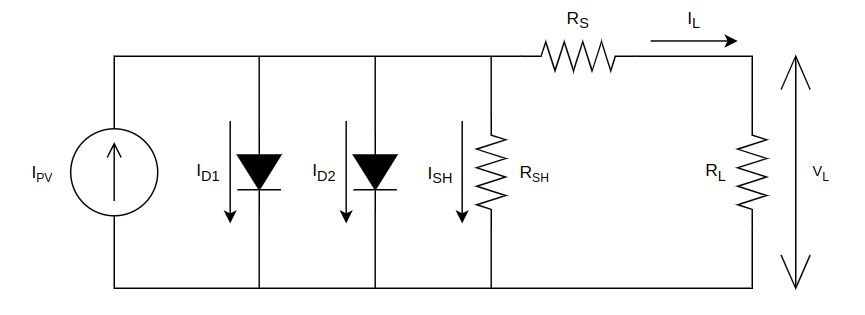
\includegraphics[width=\textwidth]{solar_cell_seven_parameter_model.png}
    \caption{Seven Parameter, or Double Diode Model of a Solar Cell}
    \label{fig:double_diode_model}
\end{figure}

The seven parameter solar cell model (\autoref{fig:double_diode_model}), also
known as a double diode model, builds upon the five parameter model by
introducing a second diode (hence the name) to more accurately model internal
current losses.

These losses can be split into the following:

\begin{itemize}
    \item losses due to carrier recombination in the space charge region of the
    P-N junction,
    \item and losses due to surface recombination.
\end{itemize}

These currents are denoted as \acf{ID1} and \acf{ID2}, respectively. By
differentiating between the two primary recombination processes in the cell, the
seven parameter model is generally considered more accurate than the five
parameter model.

The general form of this equation is shown in \autoref{eq:cell_output_current_7}.

\begin{equation}
    I_L = I_{PV} - I_{D1} - I_{D2} - I_{SH}
    \equnit{\si{\ampere}}
    \label{eq:cell_output_current_7}
\end{equation}

This results in the \autoref{eq:cell_output_current_8} when all components have
been inserted:

\begin{equation}
    \begin{split}
        I_L(V_L, G, T_C) &= I_{PV}(G, T_C, R_S, R_{SH})
                          - I_{D1}(V_L, G, T_C, R_S)
                          - I_{D2}(V_L, G, T_C, R_S) \\
        & \quad           - I_{SH}(R_S, R_{SH}) \\
        &                 = I_{SC}(G, T_C)\frac{R_S + R_{SH}}{R_{SH}}
                          - I_{01}(G, T_C)[\exp(\frac{q[V_L + I_L R_S]}{n_1 k_B T_C}) - 1] \\
        & \quad           - I_{02}(G, T_C)[\exp(\frac{q[V_L + I_L R_S]}{n_2 k_B T_C}) - 1]
                          - \frac{V_L + I_L R_S}{R_{SH}} \\
        &                 = I_{SC}(G, T_C)\frac{R_S + R_{SH}}{R_{SH}}
                          - I_{SC}(G, T_C)\frac{\exp(\frac{q[V_L + I_L R_S]}{n_1 k_B T_C}) - 1}{\exp(\frac{qV_{OC}(G, T_C)}{n_1 k_B T_C}) - 1} \\
        & \quad           - I_{SC}(G, T_C)\frac{\exp(\frac{q[V_L + I_L R_S]}{n_2 k_B T_C}) - 1}{\exp(\frac{qV_{OC}(G, T_C)}{n_2 k_B T_C}) - 1}
                          - \frac{V_L + I_L R_S}{R_{SH}} \\
        &                 = I_{SC}(G, T_C)[
                                \frac{R_S + R_{SH}}{R_{SH}}
                              + \frac{1 - \exp(\frac{q[V_L + I_L R_S]}{n_1 k_B T_C})}{1 - \exp(\frac{qV_{OC}(G, T_C)}{n_1 k_B T_C})} \\
        & \quad               + \frac{1 - \exp(\frac{q[V_L + I_L R_S]}{n_2 k_B T_C})}{1 - \exp(\frac{qV_{OC}(G, T_C)}{n_2 k_B T_C})}]
                          - \frac{V_L + I_L R_S}{R_{SH}}
    \end{split}
    \equnit{\si{\ampere}}
    \label{eq:cell_output_current_8}
\end{equation}

We note in this equation \ac{VT} was substituted back in to demonstrate that
each ideality constant for each diode is unique.

\newpage
\todo[inline]{Behold! True evil!!!\newline Not for general consumption.}
\begin{equation}
    \begin{split}
        I_L(V_L, G, T_C) &= I_{SC,ref}\frac{G}{G_{ref}}[1 - \alpha(T_{C,ref} - T_C)] \\
        & \quad             [ \\
        & \quad\quad            \frac{R_{S,ref} \exp(\zeta [T_{C,ref} - T_C])[1 + \eta(G - G_{ref})]}{R_{SH,ref} \exp(\kappa [T_{C,ref} - T_C])[1 - \iota(G - G_{ref})]} + 1 \\
        & \quad\quad          + \frac{1 - \exp(\frac{q[V_L + I_L R_{S,ref} \exp(\zeta [T_{C,ref} - T_C])[1 + \eta(G - G_{ref})]]}{n_1 k_B T_C})}{1 - \exp(\frac{q[V_{OC,ref}[1 - \beta (T_{C,ref} - T_C)] + \frac{nk_B(T_{C,ref} + T_C/\gamma)}{q}\ln(\frac{G}{G_{ref}})](G, T_C)}{n_1 k_B T_C})} \\
        & \quad\quad          + \frac{1 - \exp(\frac{q[V_L + I_L R_{S,ref} \exp(\zeta [T_{C,ref} - T_C])[1 + \eta(G - G_{ref})]]}{n_2 k_B T_C})}{1 - \exp(\frac{q[V_{OC,ref}[1 - \beta (T_{C,ref} - T_C)] + \frac{nk_B(T_{C,ref} + T_C/\gamma)}{q}\ln(\frac{G}{G_{ref}})](G, T_C)}{n_2 k_B T_C})} \\
        & \quad             ] \\
        & \quad             - \frac{V_L + I_L R_{S,ref} \exp(\zeta [T_{C,ref} - T_C])[1 + \eta(G - G_{ref})]}{R_{SH,ref} \exp(\kappa [T_{C,ref} - T_C])[1 - \iota(G - G_{ref})]}
    \end{split}
    \equnit{\si{\ampere}}
    \label{eq:cell_output_current_9}
\end{equation}

\todo[inline]{See \url{https://www.desmos.com/calculator/69rs9uo14f} to play
around with the complete seven parameter solar cell model. Add as a figure later
on compared to experimental data.}


\subsubsection{Model Summary}\label{subsubsec:seven_param_model_summary}

\todo[inline]{Might want to look for some more novel content, or wrap this section up as
is. Nothing particularly new here besides another parameter to estimate.}



\newpage
\subsection{Evaluation of Solar Cell Models}\label{subsec:eval_solar_cell_models}

To evaluate these solar cell models and their proposed modifications, we used a
set of almost 450 Maxeon Gen III and Maxeon C60 solar cells. In the following,
we discuss how we characterized these solar cells using custom \acf{HW} and
\acf{SW} to generate a robust dataset. We'll look at the dataset distributions
and compare them against the manufacturer specifications, and finally, we'll use
these extracted parameters to compare the models with the data to determine
model accuracy and precision.


\subsubsection{Solar Cell Test Setup}\label{subsubsec:solar_cell_test_setup}

\begin{figure}[!htbp]
    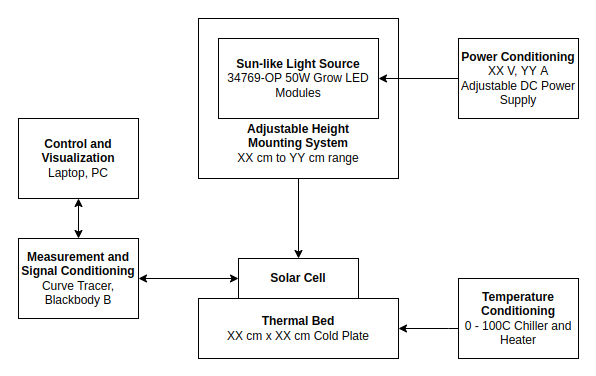
\includegraphics[width=\textwidth]{cell_test_setup.png}
    \caption{Photovoltaic Testing Setup}
    \label{fig:cell_test_setup}
\end{figure}

To characterize solar cells, we developed a test setup as outlined in
\autoref{fig:cell_test_setup}. In this test setup, we maintain three critical
requirements:

\begin{itemize}
    \item The test article experiences irradiance and temperature that is
    \textit{temporally} and \textit{spatially} uniform.
    \item The test article experiences a \textit{measurable} irradiance and
    temperature.
    \item The irradiance and temperature experienced by the test article can be
    physically manipulated.
\end{itemize}

To achieve these aforementioned requirements, we first use a solar simulator
consisting of a set of grow light modules (MPJA 34769-OPs) mounted to an
aluminum plate heatsink. The MPJA grow light modules have an emittance
spectra as shown in \autoref{fig:grow_light_spectra}; compared to the AM1.5
solar spectra (in particular, ASTMG173) in \autoref{fig:solar_spectra}, it can
be said that these LEDs are not a great characterization of natural sunlight.
A proposed design of a multi-channel LED based solar simulator is presented in
\autoref{appendix:solar_simulator}, following after similar efforts by
others~\cites{lopez_fraguas_et_al,plyta_et_al,al_ahmad_et_al,naskari_et_al},
but that is beyond the scope of this thesis.

\begin{figure}[!htbp]
    \centering
    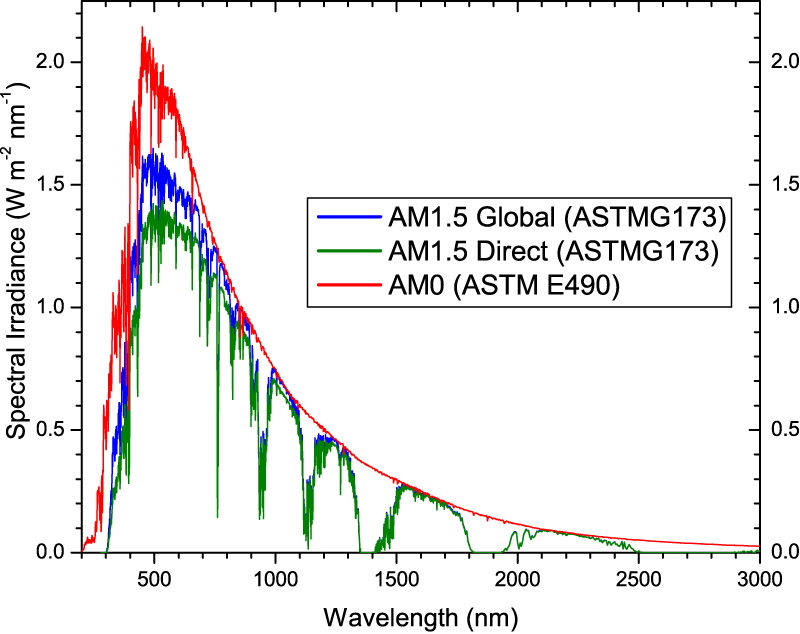
\includegraphics[width=0.65\textwidth]{solar_spectra.png}
    \caption{AM0, AM1.5 Solar Spectra}
    \label{fig:solar_spectra}
\end{figure}

\begin{figure}[!htbp]
    \centering
    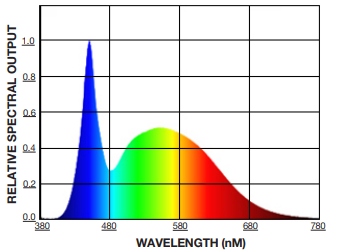
\includegraphics[width=0.65\textwidth]{mpja_grow_light_spectra.png}
    \caption{MPJA Grow Light Spectrum}
    \label{fig:grow_light_spectra}
\end{figure}

\begin{figure}[!htbp]
    \centering
    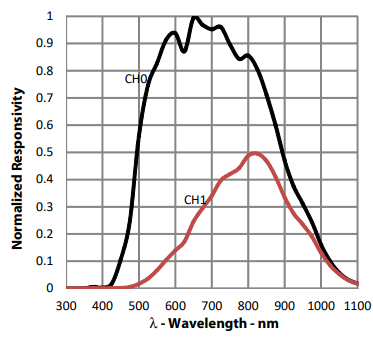
\includegraphics[width=0.65\textwidth]{tsl2591_spectral_responsivity.png}
    \caption{TSL2591 Spectral Responsivity}
    \label{fig:tsl2591_spectral_responsivity}
\end{figure}
\todo[inline]{Add reference to AMS TSL2591 datasheet. Figure 11.}

To ensure that the solar simulator irradiance is temporally uniform, a low
cost luminosity sensor (TSL2591) is used to measure the irradiance over a fixed
period of time. This period of time should be long enough to determine whether
the lights have a warm up time and change in irradiance over the expected
experiment duration. In order to get irradiance, we must convert the TSL2591
`counts' into $\si{watt}/\si{\meter}^2$; this is not straightforward, since
the normalized responsivity spectrum of the TSL2591
(\autoref{fig:tsl2591_spectral_responsivity}) is also quite divergent from
AM1.5G solar spectrum. It is, however, relatively close to the absorbance
spectra observed by the Maxeon Gen III solar cells, so the irradiance measured
by the device will closely match (if not slightly undershoot) the expected value
captured by the cell. A further discussion on methods to calibrate the sensor
readings for a true observed solar spectra is presented in
\autoref{appendix:tsl2591_calibration}. These calibration methods are useful for
testing photovoltaics outdoors.

To ensure the solar simulator irradiance is spatially uniform, the lighting
modules relative to each other and relative to the plate need to be spaced
appropriately. The light modules have a nonuniform intensity profile (e.g. light
is concentrated radially from the center of the fixture), and thus require some
overlap in illuminance area to create a superimposed, roughly uniform light
distribution. The spacing is empirically evaluated by also using the TSL2591,
similar to how \acf{PPFD} is measured~\cite{ppfd_measurement}: a closely spaced
set of points is mapped to their respective intensity measurements to
determine the variance in intensity and the lights are moved closer/farther
apart accordingly to minimize said variance.

The photovoltaic, a solar cell or solar module of up to $500 \si{\mm}$ by $250
\si{mm}$ (equivalent to 4 cells by 2 cells) in size, is placed upon a thermal
bed separated by a thin, electrically insulating layer of Kapton tape; this
thermal bed maintains the photovoltaic surface temperature via conductance, and
pumped distilled water is circulated through the bed by a \todo{Insert name of
heater/ chiller device} XXX.

After controlling for the light intensity and temperature of the test article,
the actual measurement of the solar cell parameters is performed by custom
\acp{PCB} developed by the team. The primary \ac{PCB} measures the \ac{I-V}
curve of the photovoltaic by adjusting the perceived load across the terminals.
It does this by actuating a pair of high power \acfp{MOSFET}, particularly in
the ohmic region between open and short circuit. Small steps to the gate voltage
combined with a current and voltage sensor allow for high resolution
measurements of the test article. These measurements are communicated back to
the user via \ac{USB} and captured using the Python scripting language. This
allows us to communicate to the device to set measurement profiles using either
a \ac{CLI} or \ac{GUI}. A secondary \ac{PCB} containing the TSL2591 is also
hooked up to the primary \ac{PCB} via a \ac{CAN} hardware interface. This
allows us to also combine irradiance measurements with the electrical
measurements and appropriately obtain predicted parameters at \ac{STC}. A
further description of the hardware and software implementation of these two
\acp{PCB} are provided in \autoref{appendix:curve_tracer_design} and
\autoref{appendix:blackbody_design}.

These elements of the test setup are depicted in \autoref{fig:test_setup}.

\begin{figure}[!htbp]
    \centering
    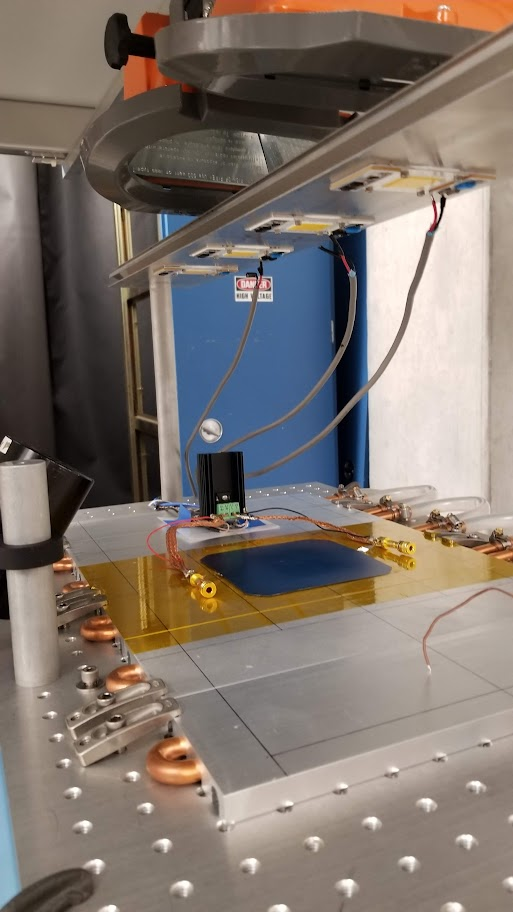
\includegraphics[trim={2cm 10cm 0cm 3cm},clip,width=0.95\textwidth]{test_setup.jpg}
    \caption{Photovoltaic Testing Setup}
    \label{fig:test_setup}
\end{figure}
\newpage


\subsubsection{Solar Cell Characterization}\label{subsubsec:solar_cell_characterization}

The actual process of characterizing solar cells is now described as follows.

\begin{enumerate}
    \item The test article is labeled with a unique identifier (e.g. BV101)
    (\autoref{fig:cell_label_placement}). This identifier is placed on the
    positive terminal of the cell, preferably in a consistent orientation, to
    facilitate quick identification and manipulation of the cell.

    \begin{figure}[!htbp]
        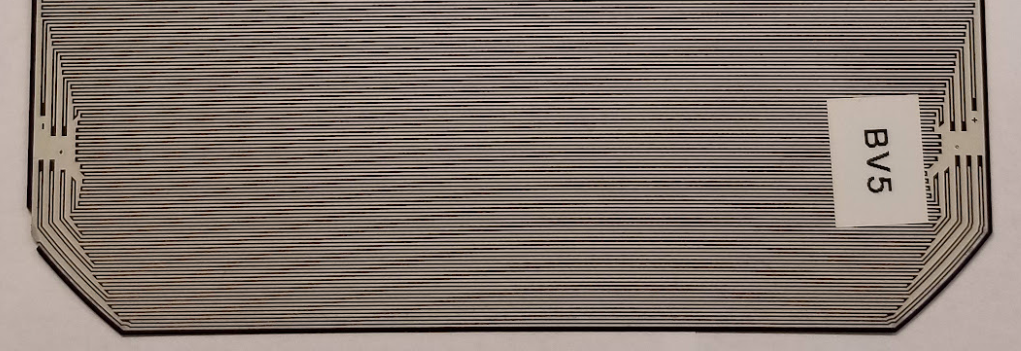
\includegraphics[width=\textwidth]{cell_label_placement.png}
        \caption{Solar Cell Label Placement}
        \label{fig:cell_label_placement}
    \end{figure}

    \item Leads are soldered on to the edge contacts of the test article, taking
    care to make sure that there are no solder bumps left after soldering nor
    excess solder bridging traces, causing a short
    (\autoref{fig:cell_with_leads}).

    \begin{figure}[!htbp]
        \missingfigure[figwidth=\textwidth]{Solar Cell with Leads Soldered On}
        \caption{Solar Cell with Leads Soldered On}
        \label{fig:cell_with_leads}
    \end{figure}

    \item The test article is placed on top of the kapton tape layer in the test
    setup, centering the article to the guide lines marked that correspond to
    the positions of the abovehead grow lights (\autoref{fig:cell_placement}).

    \begin{figure}[!htbp]
        \missingfigure[figwidth=\textwidth]{Solar Cell Placement}
        \caption{Solar Cell Placement}
        \label{fig:cell_placement}
    \end{figure}

    \item The primary \ac{PCB} connects four wires to the cell leads; two thick
    wires for current measurement and two thin wires for voltage measurement
    (\autoref{fig:cell_lead_connections}).

    \begin{figure}[!htbp]
        \missingfigure[figwidth=\textwidth]{Solar Cell Lead Connections}
        \caption{Solar Cell Lead Connections}
        \label{fig:cell_lead_connections}
    \end{figure}

    \item The primary \ac{PCB} is connected via \ac{USB} to a computer with our
    custom application installed (\autoref{fig:pcb_hookup}).

    \begin{figure}[!htbp]
        \missingfigure[figwidth=\textwidth]{\ac{PCB} Hookup}
        \caption{\ac{PCB} Hookup}
        \label{fig:pcb_hookup}
    \end{figure}

    \item We specify the conditions of the test (e.g. \ac{PV} identifier, type
    of \ac{PV}, step size, sample averaging control, test duration, etc) and
    initialize the \ac{PCB} (\autoref{fig:user_application_gui}).

    \begin{figure}[!htbp]
        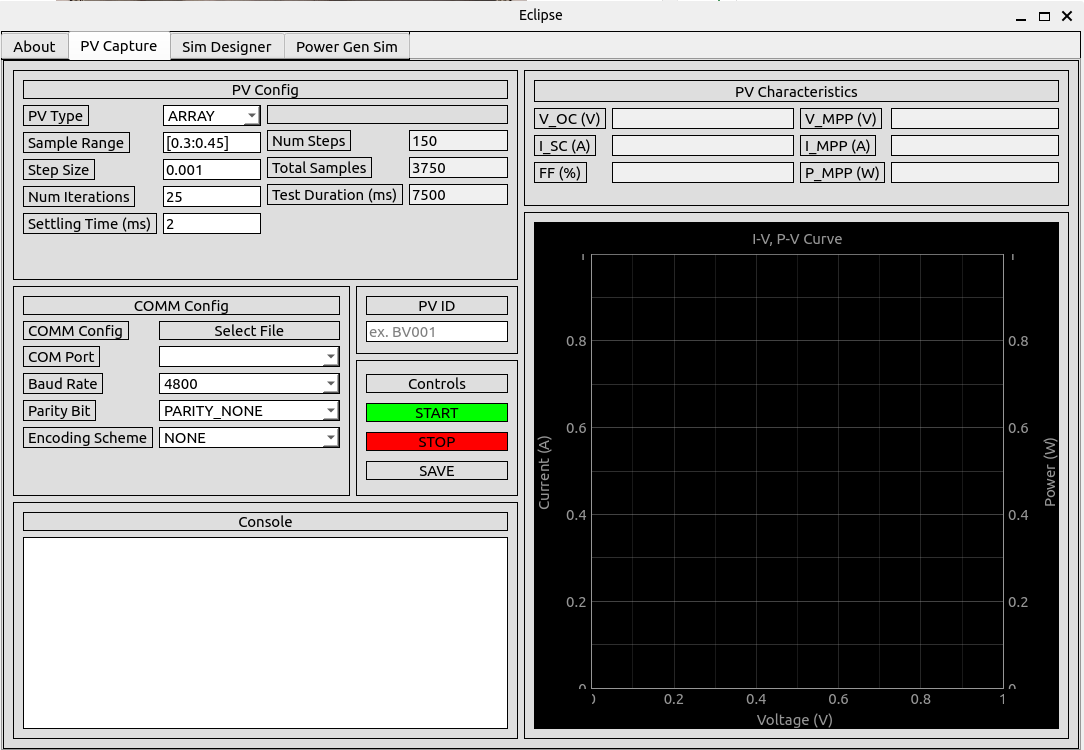
\includegraphics[width=\textwidth]{user_application_gui.png}
        \caption{User Application \ac{GUI}}
        \label{fig:user_application_gui}
    \end{figure}

    \item We enable the lighting and thermal conditioning equipment, modifying
    irradiance and temperature as expected (\autoref{fig:equipment_setup}).

    \begin{figure}[!htbp]
        \missingfigure[figwidth=\textwidth]{Equipment Setup}
        \caption{Equipment Setup}
        \label{fig:equipment_setup}
    \end{figure}

    \item We start the \ac{PCB}, which begins a scan of the \ac{PV} for the
    specified duration. The application then proceeds to capture the data from
    the \ac{PCB} and visualize it as well as extract important parameters from
    cell (\autoref{fig:cell_results}).

    \begin{figure}[!htbp]
        \missingfigure[figwidth=\textwidth]{Cell Results}
        \caption{Cell Results}
        \label{fig:cell_results}
    \end{figure}

    \item Finally, the lighting and thermal conditioning equipment are turned
    off, the cell is disconnected from the setup, and the leads are desoldered.
\end{enumerate}

An optional action is that we can hook up the secondary \ac{PCB} that measures
the irradiance from the test setup prior to placing the solar cell
(\autoref{fig:secondary_pcb_hookup}). This allows the primary \ac{PCB} to also
return the expected cell irradiance to the user application, which will
automatically adjust and predict the curve at \ac{STC}
(\autoref{fig:cell_results_normalized}).

\begin{figure}[!htbp]
    \missingfigure[figwidth=\textwidth]{Secondary PCB Hookup}
    \caption{Secondary PCB Hookup}
    \label{fig:secondary_pcb_hookup}
\end{figure}

\begin{figure}[!htbp]
    \missingfigure[figwidth=\textwidth]{Cell Results Normalized}
    \caption{Cell Results Normalized}
    \label{fig:cell_results_normalized}
\end{figure}


\subsubsection{Extraction of Cell Parameters}\label{subsubsec:extraction_of_cell_parameters}

\todo[inline,caption={}]{
    \begin{enumerate}
        \item Scatter plot of \ac{I-V}, \ac{P-V} curves
        \item Review of parameters that need to be measured:
        \begin{itemize}
            \item \acf{G}
            \item \acf{TC}
            \item \acf{VOC}
            \item \acf{ISC}
            \item \acf{RS}
            \item \acf{RSH}
            \item \acf{ALPHA}
            \item \acf{BETA}
            \item \acf{ZETA}
            \item \acf{ETA}
            \item \acf{KAPPA}
            \item \acf{IOTA}
            \item \acf{N1}
            \item \acf{N2}
            \item \acf{GAMMA}
        \end{itemize}
        \item Empirical Measurement of \ac{G} to \ac{RSH}
        \item Empirical Measurement of \ac{ALPHA} to \ac{IOTA}
        \item Statistical Measurement of \ac{N1} to \ac{GAMMA}
        \item Evaluation of parameter distributions
        \item Comparison of distribution against smith et al~\cite{smith_et_al}
    \end{enumerate}
}


\subsubsection{Solar Cell Dataset}\label{subsubsec:solar_cell_dataset}

The solar cells used for the \ac{LHRs} solar vehicle are a mixture of Maxeon Gen
III and Maxeon C60 solar cells. These solar cells were selected primarily due to
financial and availability constraints; historically, in the last two solar
vehicle revisions (2018, 2021) Gen III Bin Le1 cells have been used, but this
year the team decided to procure cheaper, more easily available C60 cells from
secondary suppliers. Regardless, these cell lines remain state of the art
despite their age\footnote{the dates are unclear, but it appears that C60 was
introduced around 2007~\cite{sunpower_history} and the Gen III has been around
as long as 2013~\cite{smith_et_al}.}; both Aptera
Motors~\cite{aptera_solar_cells} and Lightyear
One~\cite{lightyear_one_solar_cells} -the latter of which is a former
competitive solar vehicle team- have announced cooperation with Maxeon to use
their solar cells. Aptera in particular uses the Gen III
cells~\cite{aptera_solar_cells}.

While these cell types are both $125 \si{\mm}$ by $125 \si{mm}$ (see
\autoref{fig:maxeon_gen_iii_cell_footprint} for a visualization of the cell
physical layout), the Gen III cells are slightly more efficient than the C60
cells. Their (Gen III) rear contacts also tend to be slightly narrower than the
C60 cells. Their electrical characteristics are outlined in
\autoref{fig:maxeon_gen_iii_cell_characteristics} and
\autoref{fig:maxeon_c60_cell_characteristics}. Note that the Maxeon Gen III
cells are explicitly Bin Le1 cells, although the dataset will later show that
the binning for both groups of cells tends to not be very respective of the
actual measured \ac{I-V} curves, which is likely due to the variance in our
testing setup.

Since these cells were unpacked and designated for specific years,
\autoref{table:solar_cell_dataset} is provided to delineate between the
different types and `lines' of cells tested. `Lines' in this sense indicate
the academic year the cells were originally unpacked and tested.

\begin{figure}[!htbp]
    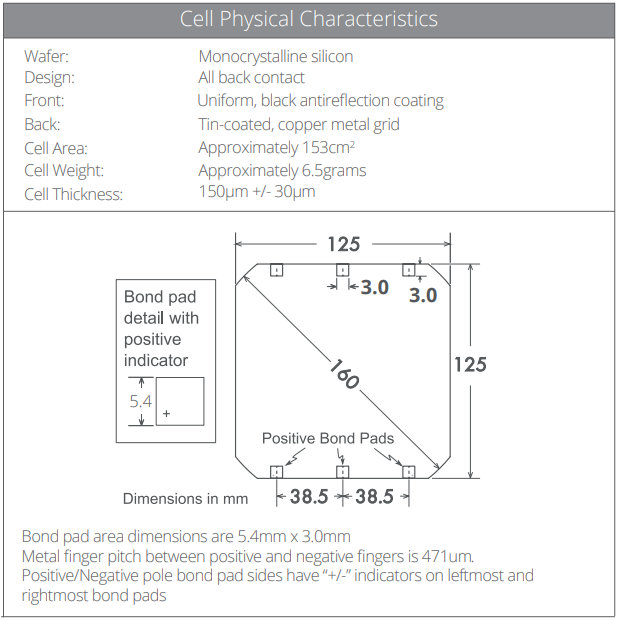
\includegraphics[width=\textwidth]{maxeon_gen_iii_cell_footprint.png}
    \caption{Maxeon Gen III Cell Footprint}
    \label{fig:maxeon_gen_iii_cell_footprint}
\end{figure}

\begin{figure}[!htbp]
    \centering
    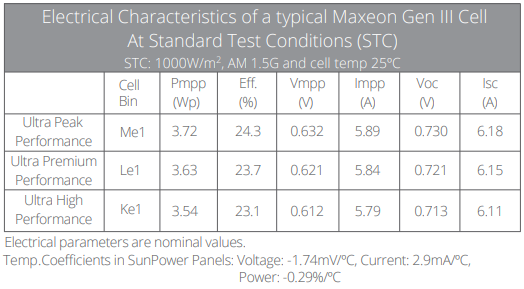
\includegraphics[width=0.95\textwidth]{maxeon_gen_iii_cell_characteristics.png}
    \caption{Maxeon Gen III Cell Characteristics}
    \label{fig:maxeon_gen_iii_cell_characteristics}
\end{figure}

\begin{figure}[!htbp]
    \centering
    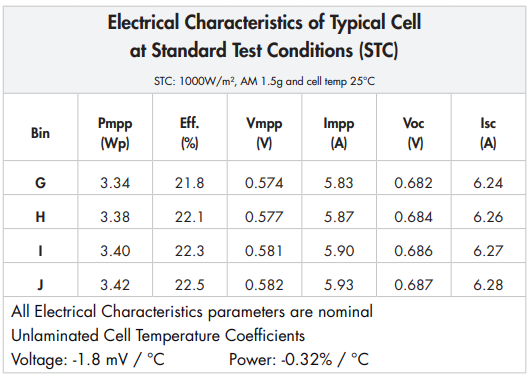
\includegraphics[width=0.95\textwidth]{maxeon_c60_cell_characteristics.png}
    \caption{Maxeon C60 Cell Characteristics}
    \label{fig:maxeon_c60_cell_characteristics}
\end{figure}

\begin{table}[!htbp]
    \begin{tabularx}{\textwidth}{
        | >{\raggedright\arraybackslash}X
        | >{\raggedright\arraybackslash}X
        | >{\raggedright\arraybackslash}X
        | >{\raggedright\arraybackslash}X | }
        \hline
        Cell Line   & Year Unpacked & Type      & Number of Cells \\ \hline \hline
        RP          & 2022          & C60       & X               \\ \hline
        MW          & 2020          & Gen III   & X               \\ \hline
        2019\_Le1   & 2019          & Gen III   & X               \\ \hline
        BU          & 2018          & Gen III   & X               \\ \hline
    \end{tabularx}
    \caption{Cell Lines Used in Solar Cell Dataset}
    \label{table:solar_cell_dataset}
\end{table}
\todo[inline]{Add number of cells tested to each group in table.}

\todo[inline,caption={}]{
    \begin{enumerate}
        \item Evaluation of parameter distributions
        \item Comparison of distributions against smith et al~\cite{smith_et_al}
    \end{enumerate}
}


\subsubsection{Modeling Solar Cell Datasets}\label{subsubsec:modeling_solar_cell_datasets}

\todo[inline,caption={}]{
    \begin{enumerate}
        \item Evaluate initial Desmos models using datasheet parameters
        \item Compare secondary Python models using extracted parameters against
        cell \ac{I-V} curves.
    \end{enumerate}
}


\subsubsection{Results}\label{subsubsec:solar_cell_model_results}

\todo[inline]{
    Holistic evaluation w/ table on statistics of model: e.g. for a
    given model and extracted cell parameters, what is the overall
    cell line accuracy and precision?
}



% TODO: Conclusion to modeling solar cells
\todo[inline]{Conclusion to modeling solar cells}

\section{Modeling Solar Modules}\label{sec:modeling_solar_modules}

After modeling the solar cell, the next layer up in the abstraction chain is
modeling a solar module. A solar module, in a typical configuration, may consist
of several solar cells in series, also called a `string'. For the \ac{LHRs}
vehicle, we place many modules in series with each other before terminating at
our variable load, a \acf{MPPT}. In our configuration, for each module, we place
a `bypass diode' in antiparallel to each module. This is used to provide an
alternative path of current to flow in the event that a solar module is
insufficient for driving the current. This could happen if a single (or several)
solar cell(s) in the module is (are) broken, or shaded, or some combination of
the two.

In this section, we'll focus on the conditions that cause issues with solar
modules, in particular, cell mismatch. We'll look at how cells with differing
operating conditions in series can drag down the efficiency of the module, and
we'll incorporate the bypass diode into the model and investigate the
conditions in which it activates and to what degree it activates.

\subsection{Modeling Photovoltaic Strings}\label{subsec:solar_cell_strings}


\begin{figure}[!htbp]
    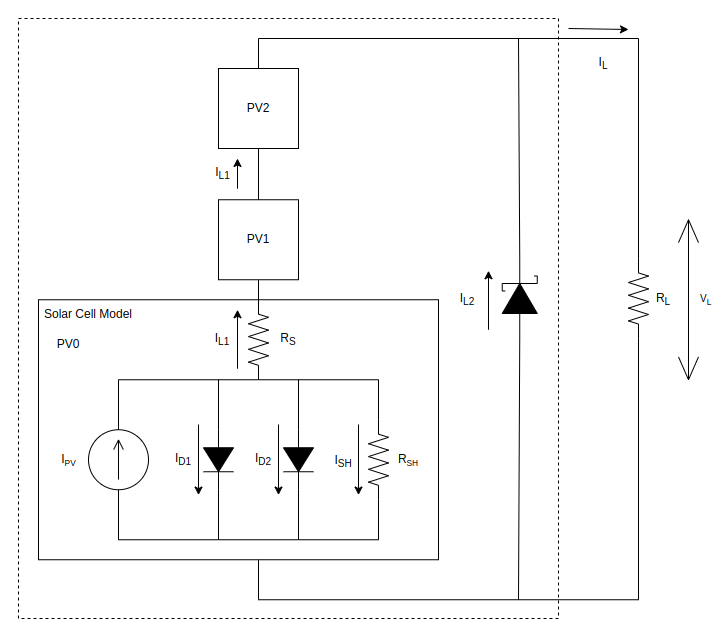
\includegraphics[width=\textwidth]{solar_module_model.png}
    \caption{Solar Module Model}
    \label{fig:solar_module_model}
\end{figure}

\subsection{Modeling Bypass Diodes}\label{subsec:bypass_diodes}

\subsection{Evaluation of Solar Module Models}\label{subsec:eval_solar_module_models}

\subsubsection{Solar Module Dataset}\label{subsubsec:solar_module_dataset}

\todo[inline,caption={}]{
    \begin{enumerate}
        \item Discussion of modules assembled, individual cell \ac{I-V} curves
        \item Discussion of lamination process (add reference to appendix for
        full procedure) and expected effect on efficiency
        \item
    \end{enumerate}
}

\subsubsection{Solar Module Test Setup}\label{subsubsec:solar_module_test_setup}

\todo[inline]{Refer to cell test setup and modifications for solar modules}


\subsubsection{Modeling Solar Module Datasets}\label{subsubsec:modeling_solar_module_datasets}

\todo[inline]{
    Compare Python model using extracted parameters against module \ac{I-V}
    curves.
}


\subsubsection{Evaluation of Solar Module Model}\label{subsubsec:evaluation_of_solar_module_model}

\todo[inline]{
    Holistic evaluation w/ table on statistics of model: e.g. for the model and
    extracted module parameters, what is the overall module accuracy and
    precision?
}


\section{Modeling Solar Arrays}\label{sec:modeling_solar_arrays}

Finally, we take the solar module model developed in the previous section and
combine it with many other modules in series to form a solar array model. In
this section we will focus on the global \ac{I-V} curve generated from the solar
array, and how the overall properties of the curve change under differing
environmental conditions, namely irradiance changes and partial shading. We'll
also look at the temporal properties of a solar array model, such as how long it
takes to effectively change voltage across the solar array.

\subsection{Modeling Shading Effects}\label{subsec:shading_effects}

\newpage
\subsection{Modeling Dynamic Behaviors}\label{subsec:temporal_modeling}

\newpage
\subsection{Evaluation of Solar Array Models}\label{subsec:eval_solar_array_models}

\todo[inline]{Introduction for evaluation of solar array models.}


\subsubsection{Solar Array Test Setup}\label{subsubsec:solar_array_test_setup}

\todo[inline]{Discuss outside array testing.}


\subsubsection{Modeling Solar Array Datasets}\label{subsubsec:modeling_solar_array_datasets}

\todo[inline]{
    Compare Python model using extracted parameters against array \ac{I-V}
    curves.
}


\subsubsection{Results}\label{subsubsec:solar_array_model_results}

\todo[inline]{
    Holistic evaluation w/ table on statistics of model: e.g. for the model and
    extracted array parameters, what is the overall array accuracy and
    precision?
}



\dots
%TODO: conclusion for Chapter 1
\todo{Insert conclusion on chapter topics and results.}
